\documentclass[a4paper]{article}

\def\npart {IA}
\def\nterm {Michaelmas}
\def\nyear {2014}
\def\nlecturer {M. G. Worster}
\def\ncourse {Differential Equations}

% Imports
\ifx \nextra \undefined
  \usepackage[pdftex,
    hidelinks,
    pdfauthor={Dexter Chua},
    pdfsubject={Cambridge Maths Notes: Part \npart\ - \ncourse},
    pdftitle={Part \npart\ - \ncourse},
  pdfkeywords={Cambridge Mathematics Maths Math \npart\ \nterm\ \nyear\ \ncourse}]{hyperref}
  \title{Part \npart\ - \ncourse}
\else
  \usepackage[pdftex,
    hidelinks,
    pdfauthor={Dexter Chua},
    pdfsubject={Cambridge Maths Notes: Part \npart\ - \ncourse\ (\nextra)},
    pdftitle={Part \npart\ - \ncourse\ (\nextra)},
  pdfkeywords={Cambridge Mathematics Maths Math \npart\ \nterm\ \nyear\ \ncourse\ \nextra}]{hyperref}

  \title{Part \npart\ - \ncourse \\ {\Large \nextra}}
\fi

\author{Lectured by \nlecturer \\\small Notes taken by Dexter Chua}
\date{\nterm\ \nyear}

\usepackage{alltt}
\usepackage{amsfonts}
\usepackage{amsmath}
\usepackage{amssymb}
\usepackage{amsthm}
\usepackage{booktabs}
\usepackage{caption}
\usepackage{enumitem}
\usepackage{fancyhdr}
\usepackage{graphicx}
\usepackage{mathtools}
\usepackage{microtype}
\usepackage{multirow}
\usepackage{pdflscape}
\usepackage{pgfplots}
\usepackage{siunitx}
\usepackage{tabularx}
\usepackage{tikz}
\usepackage{tkz-euclide}
\usepackage[normalem]{ulem}
\usepackage[all]{xy}

\pgfplotsset{compat=1.12}

\pagestyle{fancyplain}
\lhead{\emph{\nouppercase{\leftmark}}}
\ifx \nextra \undefined
  \rhead{
    \ifnum\thepage=1
    \else
      \npart\ \ncourse
    \fi}
\else
  \rhead{
    \ifnum\thepage=1
    \else
      \npart\ \ncourse\ (\nextra)
    \fi}
\fi
\usetikzlibrary{arrows}
\usetikzlibrary{decorations.markings}
\usetikzlibrary{decorations.pathmorphing}
\usetikzlibrary{positioning}
\usetikzlibrary{fadings}
\usetikzlibrary{intersections}
\usetikzlibrary{cd}

\newcommand*{\Cdot}{\raisebox{-0.25ex}{\scalebox{1.5}{$\cdot$}}}
\newcommand {\pd}[2][ ]{
  \ifx #1 { }
    \frac{\partial}{\partial #2}
  \else
    \frac{\partial^{#1}}{\partial #2^{#1}}
  \fi
}

% Theorems
\theoremstyle{definition}
\newtheorem*{aim}{Aim}
\newtheorem*{axiom}{Axiom}
\newtheorem*{claim}{Claim}
\newtheorem*{cor}{Corollary}
\newtheorem*{defi}{Definition}
\newtheorem*{eg}{Example}
\newtheorem*{fact}{Fact}
\newtheorem*{law}{Law}
\newtheorem*{lemma}{Lemma}
\newtheorem*{notation}{Notation}
\newtheorem*{prop}{Proposition}
\newtheorem*{thm}{Theorem}

\renewcommand{\labelitemi}{--}
\renewcommand{\labelitemii}{$\circ$}
\renewcommand{\labelenumi}{(\roman{*})}

\let\stdsection\section
\renewcommand\section{\newpage\stdsection}

% Strike through
\def\st{\bgroup \ULdepth=-.55ex \ULset}

% Maths symbols
\newcommand{\bra}{\langle}
\newcommand{\ket}{\rangle}

\newcommand{\N}{\mathbb{N}}
\newcommand{\Z}{\mathbb{Z}}
\newcommand{\Q}{\mathbb{Q}}
\renewcommand{\H}{\mathbb{H}}
\newcommand{\R}{\mathbb{R}}
\newcommand{\C}{\mathbb{C}}
\newcommand{\Prob}{\mathbb{P}}
\renewcommand{\P}{\mathbb{P}}
\newcommand{\E}{\mathbb{E}}
\newcommand{\F}{\mathbb{F}}
\newcommand{\cU}{\mathcal{U}}
\newcommand{\RP}{\mathbb{RP}}
\newcommand{\CP}{\mathbb{CP}}

\newcommand{\ph}{\,\cdot\,}

\DeclareMathOperator{\sech}{sech}
\DeclareMathOperator{\cosech}{cosech}
\DeclareMathOperator{\cosec}{cosec}

\DeclareMathOperator{\covol}{covol}
\DeclareMathOperator{\vol}{vol}

\let\Im\relax
\let\Re\relax
\DeclareMathOperator{\Im}{Im}
\DeclareMathOperator{\Re}{Re}
\DeclareMathOperator{\im}{im}
\DeclareMathOperator{\image}{image}
\DeclareMathOperator{\Ann}{Ann}

\DeclareMathOperator*{\res}{res}
\DeclareMathOperator{\Res}{Res}
\DeclareMathOperator{\Ind}{Ind}

\DeclareMathOperator{\tr}{tr}
\DeclareMathOperator{\diag}{diag}
\DeclareMathOperator{\rank}{rank}
\DeclareMathOperator{\card}{card}
\DeclareMathOperator{\spn}{span}
\DeclareMathOperator{\adj}{adj}

\DeclareMathOperator{\erf}{erf}
\DeclareMathOperator{\erfc}{erfc}

\DeclareMathOperator{\ord}{ord}
\DeclareMathOperator{\Sym}{Sym}

\DeclareMathOperator{\sgn}{sgn}
\DeclareMathOperator{\orb}{orb}
\DeclareMathOperator{\stab}{stab}
\DeclareMathOperator{\ccl}{ccl}

\DeclareMathOperator{\lcm}{lcm}
\DeclareMathOperator{\hcf}{hcf}

\DeclareMathOperator{\Int}{Int}
\DeclareMathOperator{\id}{id}

\DeclareMathOperator{\betaD}{beta}
\DeclareMathOperator{\gammaD}{gamma}
\DeclareMathOperator{\Poisson}{Poisson}
\DeclareMathOperator{\binomial}{binomial}
\DeclareMathOperator{\multinomial}{multinomial}
\DeclareMathOperator{\Bernoulli}{Bernoulli}
\DeclareMathOperator{\like}{like}

\DeclareMathOperator{\var}{var}
\DeclareMathOperator{\cov}{cov}
\DeclareMathOperator{\bias}{bias}
\DeclareMathOperator{\mse}{mse}
\DeclareMathOperator{\corr}{corr}

\DeclareMathOperator{\otp}{otp}
\DeclareMathOperator{\dom}{dom}

\DeclareMathOperator{\Root}{Root}
\DeclareMathOperator{\supp}{supp}
\DeclareMathOperator{\rel}{rel}
\DeclareMathOperator{\Hom}{Hom}
\DeclareMathOperator{\Aut}{Aut}
\DeclareMathOperator{\Gal}{Gal}
\DeclareMathOperator{\Mat}{Mat}
\DeclareMathOperator{\End}{End}
\DeclareMathOperator{\Char}{char}
\DeclareMathOperator{\ev}{ev}
\DeclareMathOperator{\St}{St}
\DeclareMathOperator{\Lk}{Lk}
\DeclareMathOperator{\disc}{disc}
\DeclareMathOperator{\Isom}{Isom}
\DeclareMathOperator{\length}{length}
\DeclareMathOperator{\energy}{energy}
\DeclareMathOperator{\area}{area}
\DeclareMathOperator{\Syl}{Syl}
\DeclareMathOperator{\cl}{cl}
\DeclareMathOperator{\fix}{fix}

\newcommand{\GL}{\mathrm{GL}}
\newcommand{\SL}{\mathrm{SL}}
\newcommand{\PGL}{\mathrm{PGL}}
\newcommand{\PSL}{\mathrm{PSL}}
\newcommand{\PSU}{\mathrm{PSU}}
\newcommand{\Or}{\mathrm{O}}
\newcommand{\SO}{\mathrm{SO}}
\newcommand{\U}{\mathrm{U}}
\newcommand{\SU}{\mathrm{SU}}

\renewcommand{\d}{\mathrm{d}}
\newcommand{\D}{\mathrm{D}}

\tikzset{->/.style = {decoration={markings,
                                  mark=at position 1 with {\arrow[scale=2]{latex'}}},
                      postaction={decorate}}}
\tikzset{<-/.style = {decoration={markings,
                                  mark=at position 0 with {\arrowreversed[scale=2]{latex'}}},
                      postaction={decorate}}}
\tikzset{<->/.style = {decoration={markings,
                                   mark=at position 0 with {\arrowreversed[scale=2]{latex'}},
                                   mark=at position 1 with {\arrow[scale=2]{latex'}}},
                       postaction={decorate}}}
\tikzset{->-/.style = {decoration={markings,
                                   mark=at position #1 with {\arrow[scale=2]{latex'}}},
                       postaction={decorate}}}
\tikzset{-<-/.style = {decoration={markings,
                                   mark=at position #1 with {\arrowreversed[scale=2]{latex'}}},
                       postaction={decorate}}}

\tikzset{circ/.style = {fill, circle, inner sep = 0, minimum size = 3}}
\tikzset{mstate/.style={circle, draw, blue, text=black, minimum width=0.7cm}}

\definecolor{mblue}{rgb}{0.2, 0.3, 0.8}
\definecolor{morange}{rgb}{1, 0.5, 0}
\definecolor{mgreen}{rgb}{0.1, 0.4, 0.2}
\definecolor{mred}{rgb}{0.5, 0, 0}

\def\drawcirculararc(#1,#2)(#3,#4)(#5,#6){%
    \pgfmathsetmacro\cA{(#1*#1+#2*#2-#3*#3-#4*#4)/2}%
    \pgfmathsetmacro\cB{(#1*#1+#2*#2-#5*#5-#6*#6)/2}%
    \pgfmathsetmacro\cy{(\cB*(#1-#3)-\cA*(#1-#5))/%
                        ((#2-#6)*(#1-#3)-(#2-#4)*(#1-#5))}%
    \pgfmathsetmacro\cx{(\cA-\cy*(#2-#4))/(#1-#3)}%
    \pgfmathsetmacro\cr{sqrt((#1-\cx)*(#1-\cx)+(#2-\cy)*(#2-\cy))}%
    \pgfmathsetmacro\cA{atan2(#2-\cy,#1-\cx)}%
    \pgfmathsetmacro\cB{atan2(#6-\cy,#5-\cx)}%
    \pgfmathparse{\cB<\cA}%
    \ifnum\pgfmathresult=1
        \pgfmathsetmacro\cB{\cB+360}%
    \fi
    \draw (#1,#2) arc (\cA:\cB:\cr);%
}
\newcommand\getCoord[3]{\newdimen{#1}\newdimen{#2}\pgfextractx{#1}{\pgfpointanchor{#3}{center}}\pgfextracty{#2}{\pgfpointanchor{#3}{center}}}

\def\Xint#1{\mathchoice
   {\XXint\displaystyle\textstyle{#1}}%
   {\XXint\textstyle\scriptstyle{#1}}%
   {\XXint\scriptstyle\scriptscriptstyle{#1}}%
   {\XXint\scriptscriptstyle\scriptscriptstyle{#1}}%
   \!\int}
\def\XXint#1#2#3{{\setbox0=\hbox{$#1{#2#3}{\int}$}
     \vcenter{\hbox{$#2#3$}}\kern-.5\wd0}}
\def\ddashint{\Xint=}
\def\dashint{\Xint-}


\begin{document}
\maketitle
{\small
  \noindent\textbf{Basic calculus}\\
  Informal treatment of differentiation as a limit, the chain rule, Leibnitz's rule, Taylor series, informal treatment of $O$ and $o$ notation and l'H\^opital's rule; integration as an area, fundamental theorem of calculus, integration by substitution and parts.\hspace*{\fill}[3]

  \vspace{5pt}
  \noindent Informal treatment of partial derivatives, geometrical interpretation, statement (only) of symmetry of mixed partial derivatives, chain rule, implicit differentiation. Informal treatment of differentials, including exact differentials. Differentiation of an integral with respect to a parameter.\hspace*{\fill}[2]

  \vspace{10pt}
  \noindent\textbf{First-order linear differential equations}\\
  Equations with constant coefficients: exponential growth, comparison with discrete equations, series solution; modelling examples including radioactive decay.

  \vspace{5pt}
  \noindent Equations with non-constant coefficients: solution by integrating factor.\hspace*{\fill}[2]

  \vspace{10pt}
  \noindent\textbf{Nonlinear first-order equations}\\
  Separable equations. Exact equations. Sketching solution trajectories. Equilibrium solutions, stability by perturbation; examples, including logistic equation and chemical kinetics. Discrete equations: equilibrium solutions, stability; examples including the logistic map.\hspace*{\fill}[4]

  \vspace{10pt}
  \noindent\textbf{Higher-order linear differential equations}\\
  Complementary function and particular integral, linear independence, Wronskian (for second-order equations), Abel's theorem. Equations with constant coefficients and examples including radioactive sequences, comparison in simple cases with difference equations, reduction of order, resonance, transients, damping. Homogeneous equations. Response to step and impulse function inputs; introduction to the notions of the Heaviside step-function and the Dirac delta-function. Series solutions including statement only of the need for the logarithmic solution.\hspace*{\fill}[8]

  \vspace{10pt}
  \noindent\textbf{Multivariate functions: applications}\\
  Directional derivatives and the gradient vector. Statement of Taylor series for functions on $\R^n$. Local extrema of real functions, classification using the Hessian matrix. Coupled first order systems: equivalence to single higher order equations; solution by matrix methods. Non-degenerate phase portraits local to equilibrium points; stability.

  \vspace{5pt}
  \noindent Simple examples of first- and second-order partial differential equations, solution of the wave equation in the form $f(x + ct) + g(x - ct)$.\hspace*{\fill}[5]}
\tableofcontents

\setcounter{section}{-1}
\section{Introduction}
In this course, it is assumed that students already know how to do calculus. While we will define all of calculus from scratch, it is there mostly to introduce the big and small $o$ notation which will be used extensively in this and future courses (as well as for the sake of completeness). It is impossible for a person who hasn't seen calculus before to learn calculus from those few pages.

Calculus is often used to model physical systems. For example, if we know that the force $F = m\ddot x$ on a particle at any time $t$ is given by $t^2 - 1$, then we can write this as
\[
  m\ddot x = t^2 - 1.
\]
We can easily integrate this twice with respect to $t$, and find the position $x$ as a function of time.

However, often the rules governing a physical system are not like this. Instead, the force on the particle is more likely to depend on the \emph{position} of the particle, instead of what time it is. Hence the actual equation of motion might be
\[
  m\ddot x = x^2 - 1.
\]
This is an example of a \emph{differential equation}. We are given an equation that a function $x$ obeys, often involving derivatives of $x$, and we have to find all functions that satisfy this equation (of course, the first equation is also a differential equation, but a rather boring one).

A closely related notion is \emph{difference equations}. These are discrete analogues of differential equations. A famous example is the \emph{Fibonacci sequence}, which states that
\[
  F_{n + 2} - F_{n + 1} - F_n = 0.
\]
This specifies a relationship between terms in a sequence $(F_n)$, and we want to find an explicit solution to this equation.

In this course, we will develop numerous techniques to solve different differential equations and difference equations. Often, this involves guessing of some sort.

\section{Differentiation}
We will first quickly go through basic notions of differentiation and integration. You should already be familiar with these from A levels or equivalent.

\subsection{Differentiation}
\begin{defi}[Derivative of function]
  The \emph{derivative} of a function $f(x)$ with respect to $x$, interpreted as the rate of change of $f(x)$ with $x$, is
  \[
    \frac{\d f}{\d x} = \lim_{h\to 0} \frac{f(x + h) - f(x)}{h}.
  \]
  A function $f(x)$ is differentiable at $x$ if the limit exists (ie. the left-hand and right-hand limits are equal).
\end{defi}

\begin{eg}
  $f(x)=|x|$ is not differentiable at $x = 0$ as $\lim\limits_{h\to 0^+} \frac{|h| - |0|}{h}= 1$ and $\lim\limits_{h\to 0^-} \frac{|h| - |0|}{h}= -1$.
\end{eg}

\begin{notation}
  We write $\frac{\d f}{\d x} = f'(x) = \frac{\d}{\d x} f(x)$. Also, $\frac{\d}{\d x}\left(\frac{\d}{\d x} f(x)\right) = \frac{\d^2}{\d x^2} f(x) = f''(x)$.

  Note that the notation $f'$ represents the derivative with respect to the argument. For example, $f'(2x) = \frac{\d f}{\d (2x)}$
\end{notation}

\subsection{Small \texorpdfstring{$o$}{o} and big \texorpdfstring{$O$}{O} notations}
\begin{defi}[$O$ and $o$ notations]\leavevmode
  \begin{enumerate}
    \item ``$f(x) = o(g(x))$ as $x\to x_0$'' if $\lim\limits_{x\to x_0} \frac{f(x)}{g(x)} = 0$. Intuitively, $f(x)$ is much smaller than $g(x)$.
    \item ``$f(x) = O(g(x))$ as $x\to x_0$'' if $\frac{f(x)}{g(x)}$ is bounded as $x\to x_0$. Intuitively, $f(x)$ is about as big as $g(x)$.

      Note that for $f(x) = O(g(x))$ to be true, $\displaystyle \lim_{x\to x_0} \frac{f(x)}{g(x)}$ need not exist.
  \end{enumerate}
  Usually, $x_0$ is either $0$ or infinity.
\end{defi}
Clearly, $f(x)=o(g(x))\Rightarrow f(x) = O(g(x))$.

\begin{eg}\leavevmode
  \begin{itemize}
    \item $x=o(\sqrt{x})$ as $x\to 0$ and $\sqrt{x} = o(x)$ as $x\to \infty$.
    \item $\sin 2x = O(x)$ as $x\to 0$ as $\sin \theta \approx \theta$ for small $\theta$.
    \item $\sin 2x = O(1)$ as $x\to \infty$ even though the limit does not exist.
  \end{itemize}
\end{eg}

This notation will frequently be used in calculus. For example, if we want to ignore all terms second order in $x$ in an expression, we can write out the first order terms and then append $+O(x^2)$. In particular, we can use it to characterize derivatives in a different way.
\begin{prop}
  \[
    f(x_0 + h) = f(x_0) + f'(x_0)h + o(h)
  \]
\end{prop}

\begin{proof}
  We have
  \[
    f'(x_0) = \frac{f(x_0 + h) - f(x_0)}{h} + \frac{o(h)}{h}
  \]
  by the definition of the derivative and the small $o$ notation. The result follows.
\end{proof}

\subsection{Methods of differentiation}
\begin{thm}[Chain rule]
  Given $f(x) = F(g(x))$, then
  \[
    \frac{\d f}{\d x} = \frac{\d F}{\d g}\frac{\d g}{\d x}.
  \]
\end{thm}

\begin{proof}
  Assuming that $\frac{\d g}{\d x}$ exists and is therefore finite, we have
  \begin{align*}
    \frac{\d f}{\d x} &= \lim_{h\to 0}\frac{F(g(x + h)) - F(g(x))}{h}\\
    &= \lim_{h\to 0}\frac{F[g(x) + hg'(x) + o(h)] - F(g(x))}{h}\\
    &= \lim_{h\to 0}\frac{F(g(x)) + (hg'(x) + o(h))F'(g(x)) + o(hg'(x) + o(h)) - F(g(x))}{h}\\
    &= \lim_{h\to 0}g'(x)F'(g(x)) + \frac{o(h)}{h}\\
    &= g'(x)F'(g(x))\\
    &= \frac{\d F}{\d g}\frac{\d g}{\d x}
  \end{align*}
\end{proof}

\begin{thm}[Product Rule]
  Give $f(x) = u(x)v(x)$. Then
  \[
    f'(x) = u'(x)v(x) + u(x)v'(x).
  \]
\end{thm}

\begin{thm}[Leibniz's Rule]
  Given $f = uv$, then
  \[
    f^{(n)}(x) = \sum_{r = 0}^n \binom{n}{r}u^{(r)}v^{(n - r)},
  \]
  where $f^{(n)}$ is the n-th derivative of $f$.
\end{thm}

\subsection{Taylor's theorem}
\begin{thm}[Taylor's Theorem]
  For $n$-times differentiable $f$, we have
  \[
    f(x + h) = f(x) + hf'(x) + \frac{h^2}{2!}f''(x) + \cdots + \frac{h^n}{n!}f^{(n)}(x) + E_n,
  \]
  where $E_n = o(h^{n})$ as $h\to 0$. If $f^{(n+1)}$ exists, then $E_n = O(h^{n+1})$.
\end{thm}
Note that this only gives a local approximation around $x$. This does not necessarily tell anything about values of $f$ far from $x$ (but sometimes does).

An alternative form of the sum above is:
\[
  f(x) = f(x_0) + (x-x_0)f'(x_0) + \cdots + \frac{(x-x_0)^n}{n!}f^{(n)}(x_0) + E_n.
\]
When the limit as $n\to \infty$ is taken, the Taylor series of $f(x)$ about the point $x = x_0$ is obtained.

\subsection{L'Hopital's rule}
\begin{thm}[L'Hopital's Rule]
  Let $f(x)$ and $g(x)$ be differentiable at $x_0$, and $\displaystyle \lim_{x\to x_0}f(x) = \lim_{x\to x_0}g(x) = 0$. Then
  \[
    \lim_{x\to x_0} \frac{f(x)}{g(x)} = \lim_{x\to x_0} \frac{f'(x)}{g'(x)}.
  \]
\end{thm}
\begin{proof}
  From the Taylor's Theorem, we have $f(x) = f(x_0) + (x - x_0)f'(x_0) + o(x - x_0)$, and similarly for $g(x)$. Thus
  \begin{align*}
    \lim_{x\to x_0} \frac{f(x)}{g(x)} &= \lim_{x\to x_0} \frac{f(x_0) + (x - x_0)f'(x_0) + o(x - x_0)}{g(x_0) + (x - x_0)g'(x_0) + o(x - x_0)}\\
    &= \lim_{x\to x_0} \frac{f'(x_0) + \frac{o(x-x_0)}{x-x_0}}{g'(x_0) + \frac{o(x-x_0)}{x-x_0}}\\
    &= \lim_{x\to x_0} \frac{f'(x)}{g'(x)}
  \end{align*}
\end{proof}

\section{Integration}
\subsection{Integration}
\begin{defi}[Integral]
  An \emph{integral} is the limit of a sum, eg.
  \[
    \int_a^b f(x) \;\d x = \lim_{\Delta x\to 0}\sum_{n=0}^N f(x_n)\Delta x.
  \]
  For example, we can take $\Delta x=\frac{b - a}{N}$ and $x_n = a + n\Delta x$. Note that an integral need not be defined with this particular $\Delta x$ and $x_n$. The term ``integral'' simply refers to any limit of a sum (The usual integrals we use are a special kind known as Riemann integral, which we will study formally in Analysis I). Pictorially, we have
  \begin{center}
    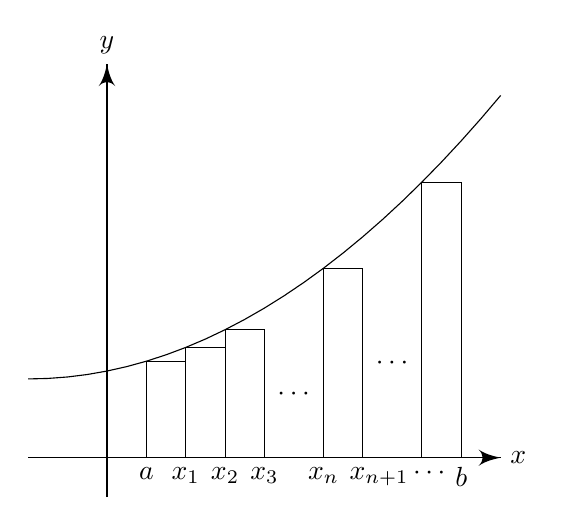
\begin{tikzpicture}
      \draw [->] (-1, 0) -- (5, 0) node [right] {$x$};
      \draw [->] (0, -0.5) -- (0, 5) node [above] {$y$};

      \draw [domain=-1:5] plot (\x, {(\x + 1)*(\x + 1)/10 + 1});

      \draw (0.5, 0) node [below] {$a$} -- (0.5, 1.225) -- (1, 1.225);
      \draw (1, 0) node [below] {$x_1$} -- (1, 1.4) -- (1.5, 1.4);
      \draw (1.5, 0) node [below] {$x_2$} -- (1.5, 1.625) -- (2, 1.625) -- (2, 0) node [below] {$x_3$};
      \node at (2.4, 0.8) {$\cdots$};
      \draw (2.75, 0) node [below] {$x_n$} -- (2.75, 2.40625) -- (3.25, 2.40625) -- (3.25, 0) node [anchor = north west] {$\!\!\!\!\!x_{n + 1}\cdots$};
      \node at (3.65, 1.2) {$\cdots$};
      \draw (4, 0) -- (4, 3.5) -- (4.5, 3.5) -- (4.5, 0) node [below] {$b$};
    \end{tikzpicture}
  \end{center}
\end{defi}

The area under the graph from $x_n$ to $x_{n+1}$ is $f(x_n)\Delta x + O(\Delta x^2)$. Provided that $f$ is differentiable, the total area under the graph from $a$ to $b$ is
\[
  \lim_{N\to \infty} \sum_{n=0}^{N-1}(f(x_n)\Delta x) + N\cdot O(\Delta x^2) = \lim_{N\to \infty} \sum_{n=0}^{N-1}(f(x_n)\Delta x) + O(\Delta x) = \int_a^b f(x)\;\d x
\]
\begin{thm}[Fundamental Theorem of Calculus]
  Let $F(x) = \int_a^x f(t)\;\d t$. Then $F'(x) = f(x)$.
\end{thm}

\begin{proof}
  \begin{align*}
    \frac{\d}{\d x}F(x) &= \lim_{h\to 0}\frac{1}{h}\left[\int_a^{x+h}f(t)\;\d t - \int_a^x f(t)\;\d t\right]\\
    &= \lim_{h\to 0} \frac{1}{h}\int_x^{x+h}f(t) \;\d t\\
    &= \lim_{h\to 0} \frac{1}{h}[f(x)h + O(h^2)]\\
    &= f(x)
  \end{align*}
\end{proof}
Similarly, we have
\[
  \frac{\d}{\d x}\int_x^b f(t)\;\d t = -f(x)
\]
and
\[
  \frac{\d}{\d x}\int_a^{g(x)} f(t)\;\d t = f(g(x))g'(x).
\]

\begin{notation}
  We write $\int f(x)\;\d x= \int^x f(t)\;\d t$, where the unspecified lower limit gives rise to the constant of integration.
\end{notation}

\subsection{Methods of integration}
Integration is substantially harder than differentiation. Given an expression, the product rule and chain rule combined with a few standard derivatives can usually differentiate it with ease. However, many seemingly-innocent expressions can turn out to be surprisingly difficult, if not impossible, to integrate. Hence we have to come up with a lot of tricks to do integrals.

\begin{eg}[Integration by substitution]
  Consider $\int \frac{1 - 2x}{\sqrt{x - x^2}}\;\d x$. Write $u = x - x^2$ and $\d u = (1 - 2x)\;\d x$. Then the integral becomes
  \[
    \int \frac{\d u}{\sqrt{u}} = 2\sqrt{u} + C = 2\sqrt{x - x^2} + C.
  \]
\end{eg}

Trigonometric substitution can be performed with reference to the following table: if the function in the 2nd column is found in the integrand, perform the substitution in the 3rd column and simplify using the identity in the first column:
\begin{center}
  \begin{tabular}{ccc}
    \toprule
    Useful identity                   & Part of integrand & Substitution      \\
    \midrule
    $\cos^2\theta + \sin^2\theta = 1$ & $\sqrt{1 - x^2}$  & $x = \sin \theta$ \\
    $1 + \tan^2\theta = \sec^2\theta$ & $1 + x^2$         & $x = \tan\theta$  \\
    $\cosh^2u - \sinh^2 u = 1$        & $\sqrt{x^2 - 1}$  & $x=\cosh u$       \\
    $\cosh^2u - \sinh^2 u = 1$        & $\sqrt{1 + x^2}$  & $x=\sinh u$       \\
    $1 - \tanh^2 u = \sech^2u$        & $1 - x^2$         & $x = \tanh u$     \\
    \bottomrule
  \end{tabular}
\end{center}
\begin{eg}
  Consider $\int \sqrt{2x - x^2}\;\d x = \int\sqrt{1 - (x - 1)^2}\;\d x$. Let $x - 1=\sin\theta$ and thus $\d x = \cos \theta\;\d\theta$. The expression becomes
  \begin{align*}
    \int \cos^2\theta \;\d \theta &= \int\frac{\cos 2\theta + 1}{2}\;\d \theta\\
    &= \frac{1}{4}\sin 2\theta + \frac{1}{2}\theta + C\\
    &= \frac{1}{2}\sin^{-1}(x - 1) + \frac{1}{2}(x - 1)\sqrt{2x - x^2} + C.
  \end{align*}
\end{eg}

\begin{thm}[Integration by parts]
  \[
    \int uv'\;\d x = uv - \int vu' \;\d x.
  \]
\end{thm}

\begin{proof}
  From the product rule, we have $(uv)' = uv' + u'v$. Integrating the whole expression and rearranging gives the formula above.
\end{proof}

\begin{eg}
  Consider $\int_0^\infty xe^{-x}\d x$. Let $u = x$ ad $v' = e^{-x}$. Then $u' = 1$ and $v = -e^{-x}$. We have
  \begin{align*}
    \int_0^\infty xe^{-x}\;\d x &= [-xe^{-x}]^\infty_0 + \int_0^\infty e^{-x} \;\d x\\
    &= 0 + [e^{-x}]_0^\infty\\
    &= 1
  \end{align*}
\end{eg}

\begin{eg}[Integration by Parts]
  Consider $\int \log x\; \d x$. Let $u = \log x$ and $v' = 1$. Then $u' = \frac{1}{x}$ and $v = x$. So we have
  \begin{align*}
    \int \log x\; \d x &= x\log x - \int \d x\\
    &= x \log x - x + C
  \end{align*}
\end{eg}

\section{Partial differentiation}
\subsection{Partial differentiation}
So far, we have only considered functions of one variable. If we have a function of multiple variables, say $f(x, y)$, we can either differentiate it with respect to $x$ or with respect to $y$.
\begin{defi}[Partial derivative]
  Given a function of several variables $f(x, y)$, the \emph{partial derivative} of $f$ with respect to $x$ is the rate of change of $f$ as $x$ varies, keeping $y$ constant. It is given by
  \[
    \left. \frac{\partial f}{\partial x}\right|_y = \lim_{\delta x\to 0} \frac{f(x + \delta x, y) - f(x, y)}{\delta x}
  \]
\end{defi}

\begin{eg}
  Consider $f(x, y) = x^2 + y^3 + e^{xy^2}$. Computing the partial derivative is equivalent to computing the regular derivative with the other variables treated as constants. eg.
  \[
    \left.\frac{\partial f}{\partial y}\right|_y = 2x + y^2e^{xy^2}.
  \]
  Second and mixed partial derivatives can also be computed:
  \begin{align*}
    \frac{\partial^2f}{\partial x^2} &= 2 + y^4e^{xy^2}\\
    \frac{\partial^2 f}{\partial y\partial x} &= \frac{\partial}{\partial y}\left(\frac{\partial f}{\partial x}\right) = 2ye^{xy^2} + 2xy^{3}e^{xy^2}
  \end{align*}
\end{eg}
It is often cumbersome to write out the variables that are kept constant. If \emph{all} other variables are being held constant, we simply don't write them out, and just say $\frac{\partial f}{\partial x}$.

Another convenient notation is
\begin{notation}
  \[
    f_x = \frac{\partial f}{\partial x},\quad f_{xy} = \frac{\partial^2 f}{\partial y\partial x}.
  \]
\end{notation}
It is important to know how the order works in the second case. The left hand side should be interpreted as $(f_x)_y$. So we first differentiate with respect to $x$, and then $y$. However, in most cases, this is not important, since we have
\begin{thm}
  If $f$ has continuous second partial derivatives, then $f_{xy} = f_{yx}$.
\end{thm}
We will not prove this statement and just assume it to be true (since this is an applied course).

\subsection{Chain rule}
Consider an arbitrary displacement in any direction $(x, y) \to (x+\delta x, y + \delta y)$. We have
\begin{align*}
  \delta f &= f(x+\delta x, y + \delta y) - f(x, y)\\
  &= f(x+\delta x, y + \delta y) - f(x + \delta x, y) + f(x+\delta x, y) - f(x, y)\\
  &= f_y(x + \delta x, y)\delta y + o(\delta y) + f_x(x, y)\delta x + o(\delta x)\\
  &= (f_x(x, y) + o(1))\delta y + o(\delta y) + f_x(x, y)\delta x + o(\delta x)\\
  \delta f&= \frac{\partial f}{\partial x}\delta x + \frac{\partial f}{\partial y}\delta y + o(\delta x, \delta y)
\end{align*}
Take the limit as $\delta x, \delta y \to 0$, we have
\begin{thm}[Chain rule for partial derivatives]
  \[
    \d f = \frac{\partial f}{\partial x}\d x + \frac{\partial f}{\partial y}\d y.
  \]
  Given this form, we can integrate the differentials to obtain the integral form:
  \[
    \int \d f = \int \frac{\partial f}{\partial x}\d x + \int \frac{\partial f}{\partial y}\d y,
  \]
  or divide by another small quantity. eg. to find the slope along the path $(x(t), y(t))$, we can divide by $\d t$ to obtain
  \[
    \frac{\d f}{\d t} = \frac{\partial f}{\partial x}\frac{\d x}{\d t} + \frac{\partial f}{\partial y}\frac{\d y}{\d t}.
  \]
\end{thm}

If we pick the parameter $t$ to be the arclength $s$, we have
\[
  \frac{\d f}{\d s} = \frac{\partial f}{\partial x}\frac{\d x}{\d s} + \frac{\partial f}{\partial y}\frac{\d y}{\d s} = \left(\frac{\d x}{\d s}, \frac{\d y}{\d s}\right)\cdot \left(\frac{\partial f}{\partial x}, \frac{\partial f}{\partial y}\right) = \hat{s}\cdot \nabla f,
\]
which is known as the directional derivative (cf. Chapter~\ref{sec:directional-derivative}).

Alternatively, the path may also be given by $y = y(x)$. So $f = f(x, y(x))$. Then the slope along the path is
\[
  \frac{\d f}{\d x} = \left.\frac{\partial f}{\partial x}\right|_y + \frac{\partial f}{\partial y}{\frac{\d y}{\d x}}.
\]
The chain rule can also be used for the change of independent variables, eg. change to polar coordinates $x = x(r, \theta)$, $y = y(r, \theta)$. Then
\[
  \left.\frac{\partial f}{\partial \theta}\right|_r = \left. \frac{\partial f}{\partial x}\right|_y \left.\frac{\partial x}{\partial \theta}\right|_r + \left.\frac{\partial f}{\partial y}\right|_x\left.\frac{\partial y}{\partial \theta}\right|_r.
\]
\subsection{Implicit differentiation}
Consider the contour surface of a function $F(x, y, z)$ given by $F(x, y, z) = $ const. This implicitly defines $z = z(x, y)$. eg. If $F(x, y, z) = xy^2 + yz^2 + z^5x = 5$, then we can have $x = \frac{5 - yz^2}{y^2 + z^5}$. Even though $z(x, y)$ cannot be found explicitly (involves solving quintic equation), the derivatives of $z(x, y)$ can still be found by differentiating $F(x, y, z) =$ const w.r.t. $x$ holding $y$ constant. eg.
\begin{align*}
  \frac{\partial }{\partial x}(xy^2 + yz^2 + z^5x) &= \frac{\partial }{\partial x}5\\
  y^2 + 2yz\frac{\partial z}{\partial x} + z^5 + 5z^4x\frac{\partial z}{\partial x} &= 0\\
  \frac{\partial z}{\partial x} &= -\frac{y^2 + z^5}{2yz + 5z^4x}
\end{align*}
In general, we can derive the following formula:
\begin{thm}[Multi-variable implicit differentiation] Given an equation
  \[
    F(x, y, z) = c
  \]
  for some constant $c$, we have
  \[
    \left.\frac{\partial z}{\partial x}\right|_y = -\frac{(\partial F)/(\partial x)}{(\partial F)/(\partial z)}
  \]
\end{thm}

\begin{proof}
  \begin{align*}
    \d F &= \frac{\partial F}{\partial x}\d x + \frac{\partial F}{\partial y}\d y + \frac{\partial F}{\partial z}\d z\\
    \left.\frac{\partial F}{\partial x}\right|_y &= \frac{\partial F}{\partial x}\left.\frac{\partial x}{\partial x}\right|_y + \frac{\partial F}{\partial y}\left.\frac{\partial y}{\partial x}\right|_y + \frac{\partial F}{\partial z}\left.\frac{\partial z}{\partial x}\right|_y = 0\\
    \frac{\partial F}{\partial x} + \frac{\partial F}{\partial z}\left.\frac{\partial z}{\partial x}\right|_y &= 0\\
    \left.\frac{\partial z}{\partial x}\right|_y &= -\frac{(\partial F)/(\partial x)}{(\partial F)/(\partial z)}
  \end{align*}
\end{proof}
\subsection{Differentiation of an integral w.r.t. parameter in the integrand}
Consider a family of functions $f(x, c)$. Define $I(b, c) = \int_0^bf(x, c)\d x$. Then by the fundamental theorem of calculus, we have $\frac{\partial I}{\partial b} = f(x, c)$. On the other hand, we have
\begin{align*}
  \frac{\partial I}{\partial c} &= \lim_{\delta c\to 0}\frac{1}{\delta c}\left[\int_0^bf(x, c + \delta c)\d x - \int_0^b f(x, c)\;\d x\right]\\
  &= \lim_{\delta c\to 0}\int_0^b\frac{f(x, c + \delta c) - f(x, c)}{\delta c}\;\d x\\
  &= \int_0^b\lim_{\delta c\to 0}\frac{f(x, c + \delta c) - f(x, c)}{\delta c}\;\d x\\
  &= \int_0^b\frac{\partial f}{\partial c}\;\d x
\end{align*}
In general, if $I(b(x), c(x)) = \int_0^{b(x)} f(y, c(x))\d y$, then by the chain rule, we have
\[
  \frac{\d I}{\d x} = \frac{\partial I}{\partial b}\frac{\d b}{\d x} + \frac{\partial I}{\partial c}\frac{\d c}{\d x} = f(b, c)b'(x) + c'(x) \int_0^b\frac{\partial f}{\partial c}\;\d y.
\]
So we obtain

\begin{thm}[Differentiation under the integral sign]
  \[
    \frac{\d}{\d x} \int_{0}^{b(x)} f(x, c(x))\;\d x= f(b, c)b'(x) + c'(x)\int_0^b \frac{\partial f}{\partial c}\;\d y
  \]
\end{thm}
This is sometimes a useful technique that allows us to perform certain otherwise difficult integrals, as you will see in the example sheets. However, here we will only have time for a boring example.

\begin{eg}
  Let $I = \int_0^1 e^{-\lambda x^2}\d x$. Then
  \[
    \frac{\d I}{\d \lambda} = \int_0^1-x^2e^{-\lambda x^2}\;\d x.
  \]
  If $I = \int_0^\lambda e^{-\lambda x^2}\d x$. Then
  \[
    \frac{\d I}{\d \lambda} = e^{-\lambda^3} + \int_0^1-x^2e^{-\lambda x^2}\;\d x.
  \]
\end{eg}

\section{First-order differential equations}
A differential equation is an equation that involves derivatives, such as $x^2\frac{\d y}{\d x} + 2y = 0$. Unlike regular equations where the solution is a number, the solution to a differential equation is a function that satisfies the equation. In this chapter, we will look at \emph{first-order differential equations}, where only first derivatives are involved.

\subsection{The exponential function}
Often, the solutions to differential equations involve the exponential function. Consider a function $f(x) = a^x$, where $a>0$ is constant.
\begin{center}
  \begin{tikzpicture}[yscale = 0.15]
    \draw [->] (-2, 0) -- (3.5, 0) node [right] {$x$};
    \draw [->] (0, -5) -- (0, 25) node [above] {$y$};

    \node [anchor = north east] at (0, 0) {$O$};
    \draw [mblue, semithick, domain=-2:3] plot (\x, {exp(\x)});
    \node [anchor = south east] at (0, 1) {1};
    \node [circ] at (0, 1) {};
  \end{tikzpicture}
\end{center}
The derivative of this function is given by
\begin{align*}
  \frac{\d f}{\d x} &= \lim_{h\to 0}\frac{a^{x+h}-a^x}{h}\\
  &= a^x\lim_{h\to 0}\frac{a^h-1}{h}\\
  &= \lambda a^x\\
  &= \lambda f(x)
\end{align*}
where $\displaystyle \lambda = \lim_{h\to 0}\frac{a^h-1}{h} = f'(0) = $ const. So the derivative of an exponential function is a multiple of the original function. In particular,

\begin{defi}[Exponential function]
  $\exp(x) = e^x$ is the unique function $f$ satisfying $f'(x) = f(x)$ and $f(0) = 1$.

  We write the inverse function as $\ln x$ or $\log x$.
\end{defi}
Then if $y = a^x = e^{x\ln a}$, then $y' = e^{x\ln a}\ln a = a^x\ln a$. So $\lambda = \ln a$.

Using this property, we find that the value of $e$ is given by
\[
  e=\lim_{k\to \infty} \left(1 + \frac{1}{k}\right)^k \approx 2.718281828\cdots.
\]
The importance of the exponential function lies in it being an \emph{eigenfunction} of the differential operator.
\begin{defi}[Eigenfunction]
  An \emph{eigenfunction} under the differential operator is a function whose functional form is unchanged by the operator. Only its magnitude is changed. ie.
  \[
    \frac{\d f}{\d x} = \lambda f
  \]
\end{defi}
\begin{eg}
  $e^{mx}$ is an eigenfunction since $\frac{\d }{\d x}e^{mx} = me^{mx}$.
\end{eg}

\subsection{Homogeneous linear ordinary differential equations}
Before we start, we will first define the terms used in the title. These are useful criteria for categorizing differential equations.

\begin{defi}[Linear differential equation]
  A differential equation is \emph{linear} if the dependent variable ($y$, $y'$, $y''$ etc.) appears only linearly.
\end{defi}

\begin{defi}[Homogeneous differential equation]
  A differential equation is \emph{homogeneous} if $y=0$ is a solution.
\end{defi}

\begin{defi}[Differential equation with constant coefficients]
  A differential equation has \emph{constant coefficients} if the independent variable $x$ does not appear explicitly.
\end{defi}

\begin{defi}[First-order differential equation]
  A differential equation is \emph{first-order} if only first derivatives are involved.
\end{defi}

\begin{thm}
  Any linear, homogeneous, ordinary differential equation with constant coefficients has solutions of the form $e^{mx}$.
\end{thm}
This theorem is evident when we consider an example.
\begin{eg}
  Given $5\frac{\d y}{\d x} - 3y = 0$. Try $y = e^{mx}$. Then
  \begin{align*}
    \frac{\d y}{\d x} &= me^{mx}\\
    5me^{mx} - 3e^{mx} &= 0
  \end{align*}
  Since this must hold for all values of $x$, there exists some value $x$ for which $e^{mx} \not= 0$ and we can divide by $e^{mx}$ (note in this case this justification is not necessary, because $e^{mx}$ is never equal to 0. However, we should justify as above if we are dividing, say, $x^m$). Thus $5m - 3 = 0$ and $m = 3/5$. So $y = e^{3x/5}$ is a solution.

  Because the equation is linear and homogeneous, any multiple of a solution is also a solution. Therefore $y = Ae^{3x/5}$ is a solution for any value of $A$.

  But is this the most general form of the solution? One can show that an $n^\text{th}$-order linear differential equation has $n$ and only $n$ independent solutions. So $y = Ae^{3x/5}$ is indeed the most general solution.
\end{eg}

We can determine $A$ by applying a given boundary condition.

\subsubsection*{Discrete equations}
Suppose that we are given the equation $5y' - 3y = 0$ with boundary condition $y = y_0$ at $x = 0$. This gives a unique function $y$. We can approximate this by considering discrete steps of length $h$ between $x_n$ and $x_{n+1}$. (Using the simple Euler numerical scheme,) we can approximate the equation by
\[
  5\frac{y_{n+1} - y_n}{h} - 3y_n \approx 0.
\]
Rearranging the terms, we have $y_{n+1} \approx (1 + \frac{3}{5}h)y_n$. Applying the relation successively, we have
\begin{align*}
  y_n &= \left(1 + \frac{3}{5}h\right)y_{n - 1}\\
  &= \left(1 + \frac{3}{5}h\right)\left(1 + \frac{3}{5}h\right)y_{n - 2}\\
  &= \left(1 + \frac{3}{5}h\right)^ny_0
\end{align*}
For each given value of $x$, choose $h = x/n$, so
\[
  y_n = y_0\left(1 + \frac{3}{5}(x/n)\right)^n.
\]
Taking the limit as $n\to \infty$, we have
\[
  y(x) = \lim_{n\to \infty} y_0\left(1 + \frac{3x/5}{n}\right)^n = y_0 e^{3x/5},
\]
in agreement with the solution of the differential equation.
\begin{center}
  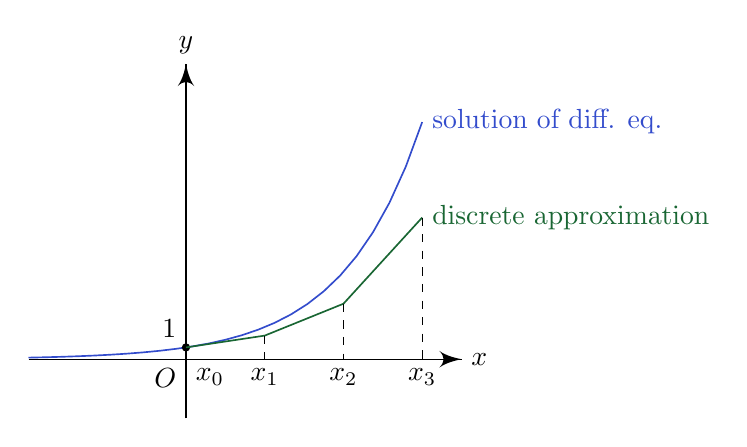
\begin{tikzpicture}[yscale = 0.15]
    \draw [->] (-2, 0) -- (3.5, 0) node [right] {$x$};
    \draw [->] (0, -5) -- (0, 25) node [above] {$y$};

    \draw [mblue, semithick, domain=-2:3] plot (\x, {exp(\x)}) node [right] {solution of diff. eq.};
    \node [anchor = south east] at (0, 1) {1};
    \node [circ] at (0, 1) {};

    \draw [mgreen, semithick] (0, 1) -- (1, 2) -- (2, 4.7) -- (3, 12) node [right] {discrete approximation};
    \draw [dashed] (1, 2) -- (1, 0);
    \draw [dashed] (2, 4.7) -- (2, 0);
    \draw [dashed] (3, 12) -- (3, 0);

    \node [anchor = north east] at (0, 0) {$O$};
    \node [anchor = north west] at (0, 0) {$x_0$};
    \node [below] at (1, 0) {$x_1$};
    \node [below] at (2, 0) {$x_2$};
    \node [below] at (3, 0) {$x_3$};
  \end{tikzpicture}
\end{center}

\subsubsection*{Series solution}
We can also try to find a solution in the form of a Taylor Series $y = \sum\limits_{n=0}^\infty a_nx^n$. We have $y' = \sum a_nnx^{n-1}$. Substituting these into our equation
\begin{align*}
  5y' - 3y &= 0\\
  5(xy')  - 3x(y) &= 0\\
  \sum a_n(5n - 3x)x^n &= 0
\end{align*}
Consider the coefficient of $x^n$: $5n a_n - 3 a_{n-1} = 0$. Since this holds for all values of $n$, when $n = 0$, we get $0a_0 = 0$. This tells that $a_0$ is arbitrary. If $n>0$, then
\[
  a_n = \frac{3}{5n}a_{n-1} = \frac{3^2}{5^2}\frac{1}{n(n-1)}a_{n-2} = \cdots = \left(\frac{3}{5}\right)^n \frac{1}{n!}a_0.
\]
Therefore we have
\[
  y = a_0\sum_{n = 0}^\infty \left(\frac{3x}{5}\right)^n\frac{1}{n!} \left[= a_0 e^{3x/5}\right].
\]

\subsection{Forced (inhomogeneous) equations}
Recall that a homogeneous equation is an equation like $5y' - 3y = 0$, with no $x$ or constant terms floating around. A forced, or inhomogeneous, equation is one that is not homogeneous. For example, $5y' - 3y = 10$ or $5y' - 3y = x^2$ are forced equations. We call the ``extra'' terms $10$ and $x^2$ the \emph{forcing terms}.

\subsubsection{Constant forcing}

\begin{eg}
  Consider $5y' - 3y = 10$. We can spot that there is a equilibrium (constant) solution $y = y_p = -\frac{10}{3}$ with $y_p' = 0$.

  The particular solution $y_p$ is a solution of the ODE. Now suppose the general solution is $y = y_p + y_c$. We see that $5y_c' - 3y_c = 0$. So $y_c$ satisfies the homogeneous equation we already solved, and
  \[
    y = -\frac{10}{3} + Ae^{3x/5}.
  \]
  Note that any boundary conditions to determine $A$ must be applied to the full solution $y$ and not the complementary function $y_c$.
\end{eg}

This is the general method of solving forced equations. We first find one particular solution to the problem, often via educated guesses. Then we solve the homogeneous equation to get a general complementary solution. Then the general solution to the full equation is the sum of the particular solution and the general complementary solution.

\subsubsection{Eigenfunction forcing}
This is the case when the forcing term is an eigenfunction of the differential operator.
\begin{eg}
  In a radioactive rock, isotope A decays into isotope B at a rate proportional to the number $a$ of remaining nuclei A, and B also decays at a rate proportional to the number $b$ of remaining nuclei B. Determine $b(t)$.

  We have
  \begin{align*}
    \frac{\d a}{\d t} &= -k_a a\\
    \frac{\d b}{\d t} &= k_a a - k_b b.
  \end{align*}
  Solving the first equation, we obtain $a = a_0e^{-k_at}$. Then we have
  \[
    \frac{\d b}{\d t} + k_b b = k_aa_0e^{-k_at}.
  \]
  We usually put the variables involving $b$ on the left hand side and the others on the right. We the right-hand term $k_aa_0e^{-k_at}$ is the \emph{forcing term}.

  Note that the forcing term is an eigenfunction of the differential operator on the LHS. So that suggests that we can try a particular integral $b_p = Ce^{-k_at}$. Substituting it in, we obtain
  \begin{align*}
    -k_aC + kB_C &= k_a a_0\\
    C &= \frac{k_a}{k_b - k_a}a_0.
  \end{align*}
  Then write $b = b_p + b_c$. We get $b'_c + k_bb_c = 0$ and $b_c = De^{-k_bt}$. All together, we have the general solution
  \[
    b = \frac{k_a}{k_b - k_a}a_0 e^{-k_at} + De^{-k_bt}.
  \]
  Assume the following boundary condition: $b = 0$ when $t = 0$, in which case we can find
  \[
    b = \frac{k_a}{k_b - k_a}a_0\left(e^{-k_at} - e^{-k_bt}\right).
  \]
  \begin{center}
    \begin{tikzpicture}[scale = 1.5]
      \draw [->] (0, 0) -- (5, 0) node [right] {$x$};
      \draw [->] (0, 0) -- (0, 3.5) node [above] {$y$};
      \node [anchor = north east] {$O$};
      \draw [domain = 0:4.5, mgreen, semithick, samples=50] plot (\x, {3*exp(-\x)});
      \draw [domain = 0:4.5, mblue, semithick, samples=50] plot (\x, {8*(exp(-\x) - exp(-1.3*\x))});
      \node [mgreen] at (0.6, 2) {$a$};
      \node [mblue] at (0.6, 0.9) {$b$};
    \end{tikzpicture}
  \end{center}
  The isotope ratio is
  \[
    \frac{b}{a} = \frac{k_a}{k_b - k_a}\left[1 - e^{(k_a - k_b)t}\right].
  \]
  So given the current ratio $b/a$, with laboratory determined rates $k_a$ and $k_b$, we can determine the value of $t$, ie. the age of the rock.
\end{eg}

\subsection{Non-constant coefficients}
Consider the general form of equation
\[
  a(x)y' + b(x)y = c(x).
\]
Divide by $a(x)$ to get the standard form
\[
  y' + p(x) y  = f(x).
\]
We solve this by multiplying an integrating factor $\mu (x)$ to obtain $(\mu)y' + (\mu p)y = \mu f$.

We want to choose a $\mu$ such that the left hand side is equal to $(\mu y)'$. By the product rule, we want $\mu p = \mu'$, ie.
\begin{align*}
  p &= \frac{1}{\mu}\frac{\d\mu }{\d x}\\
  \int p\; \d x &= \int \frac{1}{\mu}\frac{\d \mu}{\d x} \; \d x\\
  &= \int \frac{1}{\mu}\; \d u\\
  &= \ln \mu (+ C)\\
  \mu &= \exp\left(\int p\; \d x\right)
\end{align*}
Then by construction, we have $(\mu y)' = \mu f$ and thus
\[
  y = \frac{\int \mu f\;\d x}{\mu},\text{ where } \mu = \exp\left(\int p\; \d x\right)
\]
\begin{eg}
  Consider $xy' + (1 - x)y = 1$. To obtain it in standard form, we have $y' + \frac{1 - x}{x} y = \frac{1}{x}$.
  We have $\mu = \exp\left(\int (\frac{1}{x} - 1)\; \d x\right) = e^{\ln x - x} = xe^{-x}$. Then
  \begin{align*}
    y &= \frac{\int xe^{-x}\frac{1}{x}\;\d x}{xe^{-x}}\\
    &= \frac{-e^{-x} + C}{xe^{-x}}\\
    &= \frac{-1}{x} + \frac{C}{x}e^x
  \end{align*}
  Suppose that we have a boundary condition $y$ is finite at $x = 0$. Since we have $y = \frac{Ce^x - 1}{x}$, we have to ensure that $Ce^x - 1\to 0$ as $x\to 0$. Thus $C = 1$, and by L'Hopital's rule, $y\to 1$ as $x\to 0$.
\end{eg}

\subsection{Non-linear equations}
In general, a first-order equation has the form
\[
  Q(x, y)\frac{\d y}{\d x} + P(x, y) = 0.
\]
(this is not exactly the most general form, since theoretically we can have powers of $y'$ or even other complicated functions of $y'$, but we will not consider that case here).
\subsubsection{Separable equations}

\begin{defi}[Separable equation]
  A first-order differential equation is \emph{separable} if it can be manipulated into the following form:
  \[
    q(y) \;\d y = p(x) \;\d x.
  \]
  in which case the solution can be found by integration
  \[
    \int q(y)\;\d y = \int p(x)\; \d x.
  \]
\end{defi}
This is the easy kind.

\begin{eg}
  \begin{align*}
    (x^2y - 3y)\frac{\d y}{\d x} - 2xy^2 &= 4x\\
    \frac{\d y}{\d x} &= \frac{4x + 2xy^2}{x^2y - 3y}\\
    &= \frac{2x(2 +  y^2)}{y(x^2 - 3)}\\
    \frac{y}{2 + y^2}\; \d y &= \frac{2x}{x^2 - 3}\;\d x\\
    \int \frac{y}{2 + y^2}\; \d y &= \int\frac{2x}{x^2 - 3}\;\d x\\
    \frac{1}{2}\ln(2 + y^2) &= \ln (x^2 - 3) + C\\
    \ln \sqrt{2 + y^2} &= \ln A(x^2 - 3)\\
    \sqrt{y^2 + 2} &= A(x^2 - 3)
  \end{align*}
\end{eg}
\subsubsection{Exact equations}
\begin{defi}[Exact equation]
  $Q(x, y)\frac{\d y}{\d x} + P(x, y) = 0$ is an \emph{exact equation} iff the differential form $Q(x, y)\;\d y + P(x, y)\;\d x$ is \emph{exact}, ie. there exists a function $f(x, y)$ for which
  \[
    \d f = Q(x, y)\;\d y + P(x, y)\;\d x
  \]
\end{defi}

If $P(x, y)\;\d x + Q(x, y)\;\d y$ is an exact differential of $f$, then $\d f = P(x, y) \;\d x + Q(x, y)\;\d y$. But by the chain rule, $\d f  = \frac{\partial f}{\partial x}\d x + \frac{\partial f}{\partial y}\d y$ and this equality holds for any displacements $\d x, \d y$. So
\[
  \frac{\partial f}{\partial x} = P,\quad\frac{\partial f}{\partial y} = Q.
\]
From this we have
\[
  \frac{\partial^2 f}{\partial y\partial x} = \frac{\partial P}{\partial y},\quad\frac{\partial^2 f}{\partial x \partial y} = \frac{\partial Q}{\partial x}.
\]
We know that the two mixed 2nd derivatives are equal. So
\[
  \frac{\partial P}{\partial y} = \frac{\partial Q}{\partial x}.
\]
The converse is not necessarily true. Even if this equation holds, the differential need not be exact. However, it is true if the domain is \emph{simply-connected}.
\begin{defi}[Simply-connected domain]
  A domain $\mathcal{D}$ is simply-connected if it is connected and any closed curve in $\mathcal{D}$ can be shrunk to a point in $\mathcal{D}$ without leaving $\mathcal{D}$.
\end{defi}

\begin{eg}
  A disc in 2D is simply-connected. A disc with a ``hole'' in the middle is not simply-connected because a loop around the hole cannot be shrunk into a point. Similarly, a sphere in 3D is simply-connected but a torus is not.
\end{eg}

\begin{thm}
  If $\frac{\partial P}{\partial y} = \frac{\partial Q}{\partial x}$ through a simply-connected domain $\mathcal{D}$, then $P\;\d x + Q\; \d y$ is an exact differential of a single-valued function in $\mathcal{D}$.
\end{thm}
If the equation is exact, then the solution is simply $f = $ constant, and we can find $f$ by integrating $\frac{\partial f}{\partial x} = P$ and $\frac{\partial f}{\partial y} = Q$.

\begin{eg}
  \[
    6y(y - x)\frac{\d y}{\d x} + (2x - 3y^2) = 0.
  \]
  We have
  \[
    P = 2x - 3y^2, \quad Q = 6y(y - x).
  \]
  Then $\frac{\partial P}{\partial y} = \frac{\partial Q}{\partial x} = -6y$. So the differential form is exact. We now have
  \[
    \frac{\partial f}{\partial x} = 2x - 3y^2, \quad \frac{\partial f}{\partial y} = 6y^2 - 6xy.
  \]
  Integrating the first equation, we have
  \[
    f = x^2 - 3xy^2 + h(y).
  \]
  Note that since it was a partial derivative w.r.t. $x$ holding $y$ constant, the ``constant'' term can be any function of $y$. Differentiating the derived $f$ w.r.t $y$, we have
  \[
    \frac{\partial f}{\partial y} = -6xy + h'(y).
  \]
  Thus $h'(y) = 6y^2$ and $h(y) = 2y^3 + C$, and
  \[
    f = x^2 - 3xy^2 + 2y^3 + C.
  \]
  Since the original equation was $\d f = 0$, we have $f = $ constant. Thus the final solution is
  \[
    x^2 - 3xy^2 + 3y^3 = C.
  \]
\end{eg}

\subsection{Solution curves (trajectories)}
\begin{eg}
  Consider the first-order equation
  \[
    \frac{\d y}{\d t} = t(1 - y^2).
  \]
  We can solve it to obtain
  \begin{align*}
    \frac{\d y}{1 - y^2} &= t\; \d t\\
    \frac{1}{2}\ln\frac{1 + y}{1 - y} &= \frac{1}{2}t^2 + C\\
    \frac{1 + y}{1 - y} &= Ae^{t^2}\\
    y &= \frac{A - e^{-t^2}}{A + e^{-t^2}}
  \end{align*}
  We can plot the solution for different values of $A$ and obtain the following graph:
  \begin{center}
    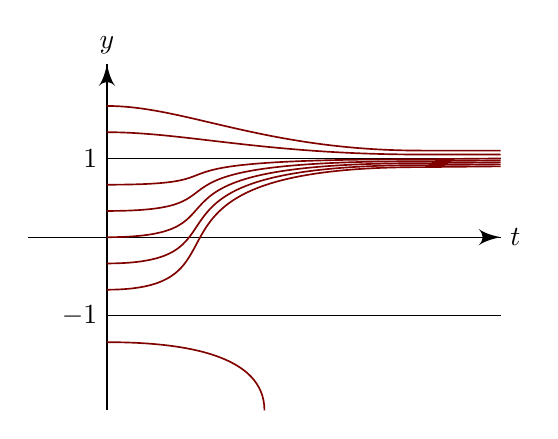
\begin{tikzpicture}
      \draw [->] (-1, 0) -- (5, 0) node [right] {$t$};
      \draw [->] (0, -2.2) -- (0, 2.2) node [above] {$y$};

      \draw (0, -1) node [left] {$-1$} -- (5, -1);
      \draw (0, 1) node [left] {$1$} -- (5, 1);

      \foreach \t in {-2,...,2} {
        \pgfmathsetmacro{\a}{0.33333 * \t};
        \pgfmathsetmacro{\b}{0.95 + .025 * \t};
        \draw [semithick, mred] (0, \a) .. controls (2, \a) and (0, \b - 0.01) .. (4, \b - 0.01) -- (5, \b);
      }
      \draw [semithick, mred] (0, -1.33333) .. controls (1, -1.33333) and (2, -1.5) .. (2, -2.2);
      \draw [semithick, mred] (0, 1.66666) .. controls (1, 1.66666) and (2, 1.1) .. (4, 1.1) -- (5, 1.1);
      \draw [semithick, mred] (0, 1.33333) .. controls (1, 1.33333) and (2, 1.05) .. (4, 1.05) -- (5, 1.05);
    \end{tikzpicture}
  \end{center}
\end{eg}

But can we understand the nature of the family of solutions without solving the equation? Can we sketch the graph without solving it?

We can spot that $y = \pm 1$ are two constant solutions and we can plot them first. We also note (and mark on our graph) that $y' = 0$ at $t = 0$ for any $y$.

Then notice that for $t > 0$, $y' > 0$ if $-1 < y < 1$. Otherwise, $y' < 0$.

Now we can find \emph{isoclines}, which are curves along which $\frac{\d y}{\d t}$ (ie. $f$) is constant: $t(1 - y^2) = D$ for some constant $D$. Then $y^2 = 1 - D/t$. After marking a few isoclines, can sketch the approximate form of our solution:
\begin{center}
  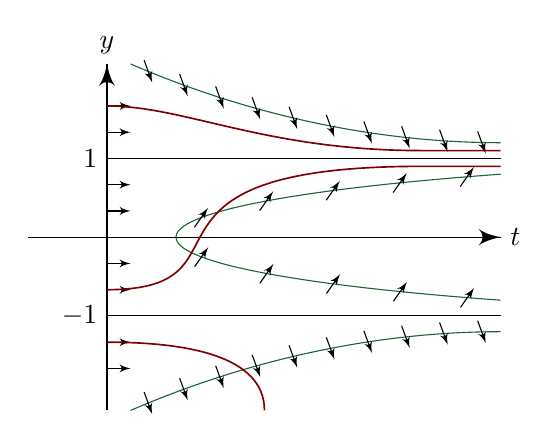
\begin{tikzpicture}
    \def\arrowlength{0.3}
    \tikzset{isocline/.style = {
      mgreen,
      decoration = {
        markings,
        mark=between positions 0.05 and 1 step 0.1 with {
          \pgftransformresetnontranslations
          \pgftransformrotate{#1}
          \draw [black, arrows={-latex'}] (-\arrowlength/2, 0) -- +(\arrowlength, 0);
        }
      },
      postaction={decorate}
    }};

    \draw [->] (-1, 0) -- (5, 0) node [right] {$t$};
    \draw [->] (0, -2.2) -- (0, 2.2) node [above] {$y$};

    \draw (0, -1) node [left] {$-1$} -- (5, -1);
    \draw (0, 1) node [left] {$1$} -- (5, 1);

    \draw [isocline=55] (5, 0.8) .. controls (-0.5, 0.4) and (-0.5, -0.4) .. (5, -0.8);
    \draw [isocline=-70] (0.3, 2.2) parabola [bend at end] (5, 1.2);
    \draw [isocline=-70] (0.3, -2.2) parabola [bend at end] (5, -1.2);

    \foreach \y in {-1.66666, -1.33333, -0.66666, -0.33333, 0.33333, 0.66666, 1.33333, 1.66666} {
      \draw [arrows={-latex'}] (0, \y) -- +(\arrowlength, 0);
    }

    \draw [semithick, mred] (0, -0.66666) .. controls (2, -0.66666) and (0, 0.9) .. (4, 0.9) -- (5, 0.9);

    \draw [semithick, mred] (0, -1.33333) .. controls (1, -1.33333) and (2, -1.5) .. (2, -2.2);
    \draw [semithick, mred] (0, 1.66666) .. controls (1, 1.66666) and (2, 1.1) .. (4, 1.1) -- (5, 1.1);
  \end{tikzpicture}
\end{center}
In general, we sketch the graph of a differential equation
\[
  \frac{\d y}{\d t} = f(t, y)
\]
by locating constant solutions (and determining stability: see below) and isoclines.

\subsection{Fixed (equilibrium) points and stability}
\begin{defi}[Equilibrium/fixed point]
  An \emph{equilibrium point} or a \emph{fixed point} of a differential equation is a constant solution $y = c$. This corresponds to $\frac{\d y}{\d t} = 0$ for all $t$.
\end{defi}
These are usually the easiest solutions to find, since we are usually given an expression for $\frac{\d y}{\d t}$ and we can simply equate it to zero.

\begin{defi}[Stability of fixed point]
  An equilibrium is \emph{stable} if whenever $y$ is deviated slightly from the constant solution $y = c$, $y \to c$ as $t \to \infty$. An equilibrium is \emph{unstable} if the deviation grows as $t \to \infty$.
\end{defi}

The objective of this section is to study how to find equilibrium points and their stability.
\begin{eg}
  Referring to the differential equation above ($\dot y = t (1 - y^2)$), we see that the solutions converge towards $y = 1$, and this is a stable fixed point. They diverge from $y = -1$, and this is an unstable fixed point.
\end{eg}

\subsubsection{Perturbation analysis}
Perturbation analysis is used to determine stability. Suppose $y = a$ is a fixed point of $\frac{\d y}{\d t} = f(y, t)$, so $f(a, t) = 0$. Write $y = a + \varepsilon(t)$, where $\varepsilon(t)$ is a small perturbation from $y = a$. We will later assume that $\varepsilon$ is arbitrarily small. Putting this into the differential equation, we have
\begin{align*}
  \frac{\d \varepsilon}{\d t} = \frac{\d y}{\d t} &= f(a + \varepsilon, t)\\
  &= f(a, t) + \varepsilon\frac{\partial f}{\partial y}(a, t) + O(\varepsilon^2)\\
  &= \varepsilon\frac{\partial f}{\partial y}(a, t) + O(\varepsilon^2)
\end{align*}
Note that this is a Taylor expansion valid when $\varepsilon \ll 1$. Thus $O(\varepsilon^2)$ can be neglected and
\[
  \frac{\d \varepsilon}{\d t} \cong \varepsilon\frac{\partial f}{\partial y}.
\]
We can use this to study how the perturbation grows with time.

This approximation is called a linearization of the differential equation.
\begin{eg}
  Using the example $\dot y = t(1 - y^2)$ above, we have
  \[
    \frac{\partial f}{\partial y} = -2yt =
    \begin{cases}
      -2t & \text{ at } y = 1\\
      2t & \text{ at } y = -1
    \end{cases}.
  \]
  At $y = 1$, $\dot{\varepsilon} = -2t\varepsilon$ and $\varepsilon = \varepsilon_0 e^{-t^2}$. Since $\varepsilon \to 0$ as $t \to \infty$, $y \to 1$. So $y = 1$ is a stable fixed point.

  On the other hand, if we consider $y = -1$, then $\dot\varepsilon = 2t\varepsilon$ and $\varepsilon = \varepsilon_0 e^{t^2}$. Since $\varepsilon \to \infty$ as $t\to \infty$, $y = -1$ is unstable.

  Technically $\varepsilon \to \infty$ is not a correct statement, since the approximation used is only valid for small $\varepsilon$. But we can be sure that the perturbation grows (even if not $\to \infty$) as $t$ increases.
\end{eg}

\subsubsection{Autonomous systems}
Often, the mechanics of a system does not change with time. So $\dot y$ is only a function of $y$ itself. We call this an \emph{autonomous system}.

\begin{defi}[Autonomous system]
  An \emph{autonomous system} is a system in the form $\dot y = f(y)$, where the derivative is only (explicitly) dependent on $y$.
\end{defi}

Near a fixed point $y = a$, where $f(a) = 0$, write $y = a + \varepsilon(t)$. Then $\dot \varepsilon = \varepsilon\frac{\d f}{\d y}(a) = k\varepsilon$ for some constant $k$. Then $\varepsilon = \varepsilon_0 e^{kt}$. The stability of the system then depends on the solely on sign of $k$.

\begin{eg}
  Consider a chemical reaction NaOH + HCl $\rightarrow$ H$_2$O + NaCl. We have
  \begin{center}
    \begin{tabular}{lccccccc}
      \toprule
      & NaOH  & + & HCl   & $\rightarrow$ & H$_2$O & + & NaCl \\
      \midrule
      Number of molecules         & $a$   &   & $b$   &               & $c$    &   & $c$ \\
      Initial number of molecules & $a_0$ &   & $b_0$ &               & $0$    &   & $0$ \\
      \bottomrule
    \end{tabular}
  \end{center}
  If the reaction is in dilute solution, then the reaction rate is proportional to $ab$. Thus
  \begin{align*}
    \frac{\d c}{\d t} &= \lambda ab\\
    &= \lambda (a_0 - c)(b_0 - c)\\
    &= f(c)
  \end{align*}
  We can plot $\frac{\d c}{\d t}$ as a function of $c$, and wlog $a_0 < b_0$.
  \begin{center}
    \begin{tikzpicture}
      \draw [->] (-0.5, 0) -- (5, 0) node [right] {$c$};
      \draw [->] (0, -1) -- (0, 4) node [above] {$\dot c$};
      \draw [mblue, semithick] (0.5, 3) parabola bend (2.5, -1) (4.5, 3);
      \node at (1.5, 0) [anchor = north east] {$a_0$};
      \node at (3.5, 0) [anchor = north west] {$b_0$};
    \end{tikzpicture}
  \end{center}
  We can also plot a \emph{phase portrait}, which is a plot of the dependent variable only, where arrows show the evolution with time,
  \begin{center}
    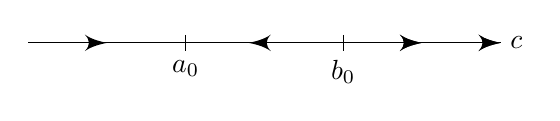
\begin{tikzpicture}
      \draw [->-=0.5] (0, 0) -- (2, 0);
      \draw [->-=0.6] (4, 0) -- (2, 0);
      \draw [->-=0.5, ->] (4, 0) -- (6, 0) node [right] {$c$};
      \draw (2, 0.1) -- (2, -0.1) node [below] {$a_0$};
      \draw (4, 0.1) -- (4, -0.1) node [below] {$b_0$};
    \end{tikzpicture}
  \end{center}
  We can see that the fixed point $c = a_0$ is stable while $c = b_0$ is unstable.

  We can also solve the equation explicitly to obtain
  \[
    c = \frac{a_0b_0[1 - e^{-(b_0 - a_0)\lambda t}]}{b_0 - a_0e^{-\lambda(b_0-a_0)t}}.
  \]
  Of course, this example makes no sense physically whatsoever because it assumes that we can have negative values of $a$ and $b$. Clearly in reality we cannot have, say, $-1$ mol of NaOH, and only solutions for $c \leq a_0$ are physically attainable, and in this case, any solution will tend towards $c = a_0$.
\end{eg}

\subsubsection{Logistic Equation}
The logistic equation is a simple model of population dynamics. Suppose we have a population of size $y$. It has a birth rate $\alpha y$ and a death rate $\beta y$. With this model, we obtain
\begin{align*}
  \frac{\d y}{\d t} &= (\alpha - \beta)y\\
  y &= y_0 e^{(\alpha - \beta)t}
\end{align*}
Our population increases or decreases exponentially depending on whether the birth rate exceeds death rate or vice versa.

However, in reality, there is fighting for limited resources. The probability of some piece of food (resource) being found is $\propto y$. The probability of the same piece of food being found by two individuals is $\propto y^2$. If food is scarce, they fight (to the death), so death rate due to fighting (competing) is $\gamma y^2$ for some $\gamma$. So
\begin{align*}
  \frac{\d y}{\d t} &= (\alpha - \beta)y - \gamma y^2\\
  \frac{\d y}{\d t}&= ry \left(1 - \frac{y}{Y}\right),
\end{align*}
where $r = \alpha - \beta$ and $Y = r/\gamma$. This is the differential logistic equation. Note that it is separable and can be solved explicitly.

However, we find the phase portrait instead. If $r = \alpha - \beta > 0$, then the graph is a quadratic parabola, and we see that $Y$ is a stable fixed point.
\begin{center}
  \begin{tikzpicture}[yscale = 1.5]
    \draw [->] (-0.5, 0) -- (4.5, 0) node [right] {$y$};
    \draw [->] (0, -1) -- (0, 2) node [above] {$f$};
    \node [anchor = north east] at (0, 0) {$O$};
    \draw [mblue, semithick] (0, 0) parabola bend (1.75, 1.5) (4, -.9796);
    \node [anchor = north east] at (3.5, 0) {$Y$};

    \draw [->-=0.5] (0, -1.5) -- (3.5, -1.5);
    \draw [-<-=0.2, ->] (3.5, -1.5) -- (4.5, -1.5) node [right] {$y$};
    \draw (0, -1.4) -- (0, -1.6) node [below] {$O$};
    \draw (3.5, -1.4) -- (3.5, -1.6) node [below] {$Y$};
  \end{tikzpicture}
\end{center}
Now when the population is small, we have
\[
  \dot y \simeq ry
\]
So the population grows exponentially. Eventually, the stable equilibrium $Y$ is reached.

\subsection{Discrete equations (Difference equations)}
Since differential equations are approximated numerically by computers with discrete equations, it is important to study the behaviour of discrete equations (and their difference with continuous counterparts).

In the logistic equation, the evolution of species may occur discretely (eg. births in spring, deaths in winter), and we can consider the population at certain time intervals (eg. consider the population at the end of each month). We might have a model in the form
\[
  x_{n + 1} = \lambda x_n(1 - x_n).
\]
This can be derived from the continuous equation with a discrete approximation
\begin{align*}
  \frac{y_{n+1} - y_n}{\Delta t} &= ry_n\left(1 - \frac{y_n}{Y}\right)\\
  y_{n + 1} &= y_n + r\Delta ty_n\left(1 - \frac{y_n}{Y}\right)\\
  &= (1 + r\Delta t)y_n - \frac{r\Delta t}{Y}y_n^2\\
  &= (1 + r\Delta t)y_n\left[1 - \left(\frac{r\Delta t}{1 + r\Delta t}\right)\frac{y_n}{Y}\right]
\end{align*}
Write
\[
  \lambda = 1 + r\Delta t,\;\;\;\;\;\; x_n = \left(\frac{r\Delta t}{1 + r\Delta t}\right)\frac{y_n}{Y},
\]
then
\[
  x_{n+1}=\lambda x_n(1 - x_n).
\]
This is the discrete logistic equation or logistic map.

If $\lambda  < 1$, then deaths exceed births and the population decays to zero.
\begin{center}
  \begin{tikzpicture}[scale=5]
    \draw [<->] (0, 1) node [above] {$x_{n + 1}$} -- (0, 0) -- (1.2, 0) node [right] {$x_n$};
    \draw [mgreen, semithick] (0, 0) -- (1, 1) node [right] {$x_{n + 1} = x_n$};
    \draw [mblue, semithick] (0, 0) parabola bend (0.5, 0.225) (1, 0);

    \draw [mred] (0.4, 0) node [below, black] {$x_0$}
    -- (0.4, 0.216) -- (0.216, 0.216)
    -- (0.216, 0.152) -- (0.152, 0.152)
    -- (0.152, 0.116) -- (0.116, 0.116)
    -- (0.116, 0.092) -- (0.092, 0.092)
    -- (0.092, 0.075) -- (0.075, 0.075);
  \end{tikzpicture}
\end{center}
We see that $x = 0$ is a fixed point.

In general, to find fixed points, we solve for $x_{n + 1} = x_n$, ie. $f(x_n) = x_n$. For the logistics map, we have
\begin{align*}
  \lambda x_n(1 - x_n) &= x_n\\
  x_n[1 - \lambda(1 - x_n)] &= 0\\
  x_n = 0 &\text{ or } x_n = 1 - \frac{1}{\lambda}
\end{align*}
When $1 < \lambda < 2$, we have
\begin{center}
  \begin{tikzpicture}[scale=5]
    \draw [<->] (0, 1) node [above] {$x_{n + 1}$} -- (0, 0) -- (1.2, 0) node [right] {$x_n$};
    \draw [mgreen, semithick] (0, 0) -- (1, 1) node [right] {$x_{n + 1} = x_n$};
    \draw [mblue, semithick] (0, 0) parabola bend (0.5, 0.45) (1, 0);

    \draw [mred] (0.2, 0) node [below, black] {$x_0$}
    -- (0.2, 0.288) -- (0.288, 0.288)
    -- (0.288, 0.369) -- (0.369, 0.369)
    -- (0.369, 0.419) -- (0.419, 0.419)
    -- (0.419, 0.438) -- (0.438, 0.438)
    -- (0.438, 0.443) -- (0.443, 0.443);
  \end{tikzpicture}
\end{center}
We see that $x_n = 0$ is an unstable fixed point and $x_n = 1 - \frac{1}{\lambda}$ is a stable fixed point.

When $2 < \lambda < 3$, we have
\begin{center}
  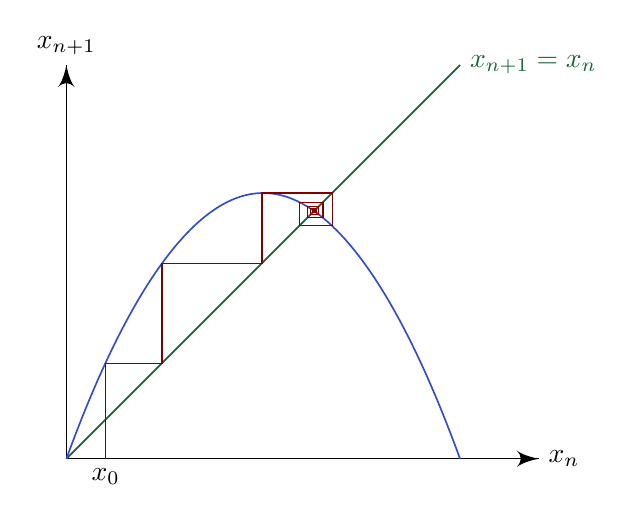
\begin{tikzpicture}[scale=5]
    \draw [<->] (0, 1) node [above] {$x_{n + 1}$} -- (0, 0) -- (1.2, 0) node [right] {$x_n$};
    \draw [mgreen, semithick] (0, 0) -- (1, 1) node [right] {$x_{n + 1} = x_n$};
    \draw [mblue, semithick] (0, 0) parabola bend (0.5, 0.675) (1, 0);

    \draw [mred] (0.1, 0) node [below, black] {$x_0$}
    -- (0.1, 0.243) -- (0.243, 0.243)
    -- (0.243, 0.497) -- (0.497, 0.497)
    -- (0.497, 0.675) -- (0.675, 0.675)
    -- (0.675, 0.592) -- (0.592, 0.592)
    -- (0.592, 0.652) -- (0.652, 0.652)
    -- (0.652, 0.613) -- (0.613, 0.613)
    -- (0.613, 0.641) -- (0.641, 0.641)
    -- (0.641, 0.621) -- (0.621, 0.621)
    -- (0.621, 0.635) -- (0.635, 0.635)
    -- (0.635, 0.626) -- (0.626, 0.626)
    -- (0.626, 0.632) -- (0.632, 0.632)
    -- (0.632, 0.628) -- (0.628, 0.628)
    -- (0.628, 0.631) -- (0.631, 0.631)
    -- (0.631, 0.629) -- (0.629, 0.629)
    -- (0.629, 0.63) -- (0.63, 0.63)
    -- (0.63, 0.629) -- (0.629, 0.629)
    -- (0.629, 0.63) -- (0.63, 0.63);
  \end{tikzpicture}
\end{center}
There is an oscillatory convergence to $x_n = 1 - \frac{1}{\lambda}$.

When $\lambda > 3$, we have a limit cycle, in which $x_n$ oscillates between 2 values, ie. $x_{n + 2} = x_n$. When $\lambda = 1 + \sqrt{6} \approx 3.449$, we have a 4-cycle, and so on.
\begin{center}
  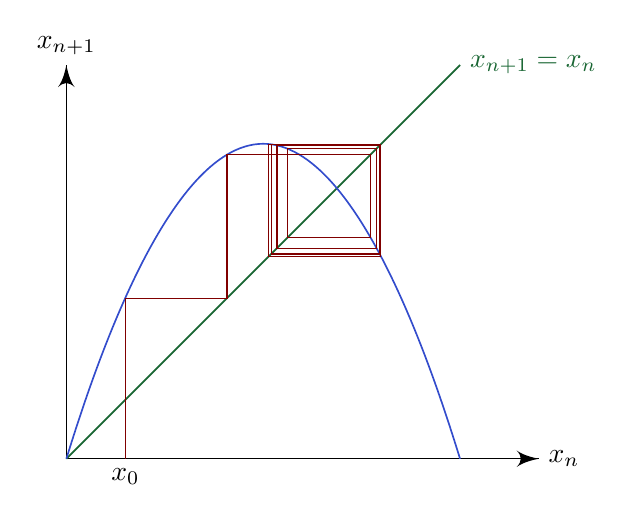
\begin{tikzpicture}[scale=5]
    \draw [<->] (0, 1) node [above] {$x_{n + 1}$} -- (0, 0) -- (1.2, 0) node [right] {$x_n$};
    \draw [mgreen, semithick] (0, 0) -- (1, 1) node [right] {$x_{n + 1} = x_n$};
    \draw [mblue, semithick] (0, 0) parabola bend (0.5, 0.8) (1, 0);

    \draw [mred] (0.15, 0) node [below, black] {$x_0$}
    -- (0.15, 0.408) -- (0.408, 0.408)
    -- (0.408, 0.773) -- (0.773, 0.773)
    -- (0.773, 0.562) -- (0.562, 0.562)
    -- (0.562, 0.788) -- (0.788, 0.788)
    -- (0.788, 0.535) -- (0.535, 0.535)
    -- (0.535, 0.796) -- (0.796, 0.796)
    -- (0.796, 0.52) -- (0.52, 0.52)
    -- (0.52, 0.799) -- (0.799, 0.799)
    -- (0.799, 0.514) -- (0.514, 0.514)
    -- (0.514, 0.799) -- (0.799, 0.799)
    -- (0.799, 0.514) -- (0.514, 0.514)
    -- (0.514, 0.799) -- (0.799, 0.799)
    -- (0.799, 0.514) -- (0.514, 0.514)
    -- (0.514, 0.799) -- (0.799, 0.799)
    -- (0.799, 0.514) -- (0.514, 0.514)
    -- (0.514, 0.799) -- (0.799, 0.799)
    -- (0.799, 0.514) -- (0.514, 0.514);
  \end{tikzpicture}
\end{center}
We can have the following plot of the stable solutions for different values of $\lambda$ (plotted as $r$ in the horizontal axis)
\begin{center}
  \includegraphics[width=330pt]{images/de_bifurcation.png}

  Credits: Wikimedia Commons: Jordan Pierce - Public Domain CC0 1.0
\end{center}
Note that the fixed point still exists after $\lambda = 3$, but is no longer stable. Similarly, the 2-cycles still exist after $\lambda = 1 + \sqrt{6}$, but it is not stable.

\section{Second-order differential equations}
We now move on to second-order differential equations. While we will only look at second-order equations, most of the methods in this section apply to higher order differential equations as well.
\subsection{Constant coefficients}
The general form of an equation with constant coefficients is
\[
  ay'' + by' + cy = f(x).
\]
We solve this in two steps:
\begin{enumerate}
  \item Find the complementary functions which satisfy the homogeneous equation $ay'' + by' + cy = 0$.
  \item Find a particular solution that satisfies the full equation.
\end{enumerate}
\subsubsection{Complementary functions}
Recall that $e^{\lambda x}$ is an eigenfunction of the differential operator $\frac{\d}{\d x}$. Hence it is also an eigenfunction of the second derivative $\frac{\d^2}{\d x^2} = \frac{\d}{\d x}\left(\frac{\d }{\d x}\right)$.

If the complementary function has the form $y_c = e^{\lambda x}$, then $y'_c = \lambda e^{\lambda x}$ and $y''_c = \lambda^2 e^{\lambda x}$. Substituting into the differential equation gives
\begin{defi}[Characteristic equation]
  The \emph{characteristic equation} of a (second-order) differential equation $ay'' + by' + c = 0$ is
  \[
    a\lambda^2 + b\lambda + c = 0.
  \]
\end{defi}

In this case there are two solutions to the characteristic equation, giving (in principle) two complementary functions $y_1 = e^{\lambda_1 x}$ and $y_2 = e^{\lambda_2 x}$.

If $\lambda_1$ and $\lambda_2$ are distinct, then $y_1$ and $y_2$ are linearly independent and complete --- they form a basis of the solution space. The (most) general complementary function is
\[
  y_c = Ae^{\lambda_1 x} + Be^{\lambda_2 x}.
\]
\begin{eg}
  $y'' - 5y' + 6y = 0$. Try $y = e^{\lambda x}$. The characteristic equation is $\lambda^2 - 5\lambda + 6 = 0$. Then $\lambda = 2$ or $3$. So the general solution is $y = Ae^{2x} + Be^{3x}$.

  Note that $A$ and $B$ can be complex constants.
\end{eg}

\begin{eg}[Simple harmonic motion]
  $y'' + 4y = 0$. Try $y = e^{\lambda x}$. The characteristic equation is $\lambda^2 + 4 = 0$, with solutions $\lambda = \pm 2i$. Then our general solution is $y = Ae^{2ix} + Be^{-2ix}$. However, if this is in a case of simple harmonic motion in physics, we want the function to be real (or \emph{look} real). We can write
  \begin{align*}
    y &= A(\cos 2x + i\sin 2x) + B(\cos 2x - i\sin 2x)\\
    &= (A + B)\cos 2x + i(A - B)\sin 2x\\
    &= \alpha\cos 2x + \beta\sin 2x
  \end{align*}
  where $\alpha = A + B$ and $\beta = i(A - B)$, and $\alpha$ and $\beta$ are independent constants.

  In effect, we have changed the basis from $\{e^{2ix}, e^{-2ix}\}$ to $\{\cos 2x$, $\sin 2x\}$.
\end{eg}

\begin{eg}[Degeneracy] $y'' - 4y' + 4y = 0$.

  Try $y = e^{\lambda x}$. We have $\lambda ^2 - 4\lambda + 4 =  0$ and $(\lambda - 2)^2 = 0$. So $\lambda = 2$ or $2$. But $e^{2x}$ and $e^{2x}$ are clearly not linearly independent. We have only managed to find one basis function of the solution space, but a second order equation has a 2 dimensional solution space. We need to find a second solution.

  We can perform \emph{detuning}. We can separate the two functions found above from each other by considering $y'' - 4y' + (4 - \varepsilon^2)y = 0$. This turns into the equation we want to solve as $\varepsilon \to 0$. Try $y = e^{\lambda x}$. We obtain $\lambda^2 - 4\lambda + 4 - \varepsilon^2$. The two roots are $\lambda = 2 \pm \varepsilon$. Then
  \begin{align*}
    y &= Ae^{(2 + \varepsilon)x} + Be^{(2 - \varepsilon)X}\\
    &= e^{2x}[A e^{\varepsilon x} + Be^{-\varepsilon x}]
    \intertext{Taking the limit as $\varepsilon \to 0$, we use the Taylor expansion of $e^{\varepsilon x}$ to obtain}
    y &= e^{2x}[(A + B) + \varepsilon x(A - B) + O(A\varepsilon^2, B\varepsilon^2)]
    \intertext{Choose $(A + B) = \alpha$ and $\varepsilon(A - B) = \beta$. This is perfectly valid for any non-zero $\varepsilon$. Then $A = \frac{1}{2}(\alpha + \frac{\beta}{\varepsilon})$ and $B = \frac{1}{2}(\alpha - \frac{\beta}{\varepsilon})$. So we have}
    y &= e^{2x}[\alpha + \beta x + O(A\varepsilon^2, B\varepsilon^2)]\\
    \intertext{Seeing $\alpha$ and $\beta$ as fixed constants independent of $\varepsilon$, $A$ and $B$ diverge as $\varepsilon \to 0$. Since $A = O(\frac{1}{\varepsilon})$, we know that  $O(A\varepsilon^2) = O(\varepsilon)$, and similarly for $B$. So}
    y &= e^{2x}[\alpha + \beta x + O(\varepsilon)]\\
    &= e^{2x}(\alpha + \beta x)
  \end{align*}
  In this way, we have derived two separate basis functions. In general, if $y_1(x)$ is a degenerate complementary function of a linear differential equation with constant coefficients, then $y_2(x) = xy_1(x)$ is an independent complementary function.
\end{eg}

\subsubsection{Second complementary function}
In general (ie. if we don't have constant coefficients), we can find a second complementary function associated with a degenerate solution of the homogeneous equation by looking for a solution in the form $y_2(x) = v(x) y_1(x)$, where $y_1(x)$ is the degenerate solution we found.

\begin{eg}
  Consider $y'' - 4y + 4y = 0$. We have $y_1 = e^{2x}$. We try $y_2 = ve^{2x}$. Then
  \begin{align*}
    y_2' &= (v' + 2v)e^{2x}\\
    y_2'' &= (v'' + 4v'' + 4v)e^{2x}.
  \end{align*}
  Substituting into the original equation gives
  \begin{align*}
    (v'' + 4v' + 4v) - 4(v' + 2v) + 4v &= 0\\
    v'' &= 0\\
    v' &= \beta\\
    v &= \alpha + \beta x.
  \end{align*}
  So $y_2 = (Ax + B)e^{2x}$.
\end{eg}

\subsubsection{Phase space}
Consider a general differential equation of $n$th order, eg.
\[
  a_n(x) y^{(n)} + a_{n - 1}y^{(n - 1)} + \cdots + a_1(x) y' + a_0 (x) y = f(x).
\]
At any point $x_0$, if we are given the first $n - 1$ derivatives, ie. $y(x_0)$, $y'(x_0)$, $\cdots$, $y^{(n - 1)}(x_0)$, we can get the $n$th derivative and also any higher derivatives from the differential equation. This means that we know the Taylor series of $y$ about $x_0$. In particular, we know how all derivatives of $y$ vary as $x$ changes.

After a small change in $x$, we arrive at a new point $x_1$. Since we know all derivatives of $y$ at this point from the initial Taylor expansion, we can use this information to know about the first $n - 1$ derivatives of $y$ at $x_1$. We can repeat this process indefinitely.

We can collect all these information about the derivatives into a \emph{solution vector} $\mathbf{Y}(x) = (y(x), y'(x),f \cdots , y^{n - 1}(x))$ for each value of $x$. Then the differential equation uniquely specifies how this solution vector $\mathbf{Y}(x)$ evolves with $x$ given an initial point $\mathbf{Y}(x_0)$. So $\mathbf{Y}(x)$ traces out a trajectory in the \emph{phase space}.

\begin{eg}
  Consider $y'' + 4y = 0$. The solutions are $y_1 = \cos 2x$ and $y_2 = \sin 2x$. Thus $y_1' = -2\sin 2x$ and $y_2' = 2\cos 2x$. The solution vectors of the complementary functions are $\mathbf{Y}_1 = (\cos 2x, -2\sin 2x)$ and $\mathbf{Y}_2 = (\sin 2x, 2\cos 2x)$. We can plot them as follows:
  \begin{center}
    \begin{tikzpicture}
      \draw [->] (-3, 0) -- (3, 0) node [right] {$y$};
      \draw [->] (0, -2) -- (0, 2) node [above] {$y'$};

      \draw (0, 0) circle [x radius = 1.2, y radius = 1.6];
      \draw [->] (0, 0) -- (1, 0.8844) node [right] {$\mathbf{Y}_1$};
      \draw [->] (0, 0) -- (0.9368, -1) node [right] {$\mathbf{Y}_2$};
    \end{tikzpicture}
  \end{center}
  with $\mathbf{Y}_1$ and $\mathbf{Y}_2$ tracing out the same curve but starting at different points.
\end{eg}

Note that this phase space is a 2-dimensional space, and we can take the two complementary functions $\mathbf{Y}_1$ and $\mathbf{Y}_2$ as basis vectors for the phase space at each particular value of $x$. Of course, we need the two solutions to be linearly independent.

\begin{defi}[Wronskian]
  Given a differential equations with solutions $y_1, y_2$, the \emph{Wronskian} is the determinant
  \[
    W(x) = \begin{vmatrix}y_1 & y_2 \\ y_1' & y_2'\end{vmatrix}.
  \]
\end{defi}
\begin{defi}[Independent solutions]
  Two solutions $y_1(x)$ and $y_2(x)$ are \emph{independent} solutions of the differential equation if and only if $\mathbf{Y}_1$  and $\mathbf{Y}_2$  are linearly independent as vectors in the phase space, ie. iff the Wronskian is non-zero.
\end{defi}

In our example, we have $W(x) = 2\cos^2 2x + 2\sin^2 2x = 2 \not= 0$ for all $x$.

\begin{eg}
  In our earlier example, $y_1 = e^{2x}$ and $y_2 = xe^{2x}$. We have
  \[
    W = \left|\begin{matrix} e^{2x} & xe^{2x}\\ 2e^{2x} & e^{2x} + 2xe^{2x} \end{matrix}\right| = e^{4x}(1 + 2x - 2x) = e^{4x} \not= 0.
  \]
\end{eg}

In both cases, the Wronskian is \emph{never} zero. Is it possible that it is zero for some $x$ while non-zero for others? The answer is no.

\begin{thm}[Abel's Theorem]
  Given an equation $y'' + p(x)y' + q(x) y = 0$, either $W = 0$ for all $x$, or $W \not= 0$ for all $x$. ie. iff two solutions are independent for some particular $x$, then they are independent for all $x$.
\end{thm}

\begin{proof}
  If $y_1$ and $y_2$ are both solutions, then
  \begin{align*}
    y_2(y_1'' + py_1' + qy_1) &= 0\\
    y_1(y_2'' + py_2' + qy_2) &= 0\\
    \intertext{Subtracting the two equations, we have}
    y_1y_2'' - y_2y_1'' + p(y_1y_2' - y_2y_1') &= 0\\
    \intertext{Note that $W =y_1y_2' - y_2y_1'$ and $W' = y_1y_2'' + y_1'y_2' - (y_2'y_1' + y_2y_1'') = y_1y_2'' - y_2y_1''$}
    W' + P(x)W &= 0\\
    W(x) &= W_0 e^{-\int P\; \d x},
  \end{align*}
  Where $W_0 = $ const. Since the exponential function is never zero, either $W_0 = 0$, in which case $W = 0$, or $W_0 \not= 0$ and $W \not= 0$ for any value of $x$.
\end{proof}
In general, any linear $n$th-order homogeneous differential equation can be written in the form $\mathbf{Y}' + A\mathbf{Y} = 0$, a system of first-order equations. It can then be shown that $W' + \tr(A)W = 0$, and $W = W_0e^{-\int \tr A\;\d x}$. So Abel's theorem holds.

\subsection{Particular integrals}
We now consider equations of the form $ay'' + by' + cy = f(x)$. We will come up with several ways to find a particular integral.

\subsubsection{Guessing}
If the forcing terms are simple, we can easily ``guess'' the form of the particular integral, as we've previously done for first-order equations.
\begin{center}
  \begin{tabular}{cc}
    \toprule
    $f(x)$ & $y_p(x)$\\
    \midrule
    $e^{mx}$ & $Ae^{mx}$\\
    $\sin kx$ & \multirow{2}{*}{$A\sin kx + B\cos kx$}\\
    $\cos kx$ & \\
    polynomial $p_n(x)$ & $q_n(x) = a_nx^n + \cdots + a_1x + a_0$\\
    \bottomrule
  \end{tabular}
\end{center}
It is important to remember that the equation is linear, so we can superpose solutions and consider each forcing term separately.

\begin{eg}
  Consider $y'' - 5y' + 6y = 2x + e^{4x}$. To obtain the forcing term $2x$, we need a first order polynomial $ax + b$, and to get $e^{4x}$ we need $ce^{4x}$. Thus we can guess
  \begin{align*}
    y_p &= ax + b + ce^{4x}\\
    y'_p &= a + 4ce^{4x}\\
    y''_p &= 16ce^{4x}
  \end{align*}
  Substituting in, we get
  \[
    16ce^{4x} - 5(a + 4ce^{4x}) + 6(ax + b + ce^{4x}) = 2x + e^{4x}
  \]
  Comparing coefficients of similar functions, we have
  \begin{align*}
    16c - 20c + 6c &= 1\Rightarrow c = \frac{1}{2}\\
    6a &= 2 \Rightarrow a = \frac{1}{3}\\
    -5a + 6b &= 0 \Rightarrow b = \frac{5}{18}
  \end{align*}
  Since the complementary function is $y_c = Ae^{3x} + Be^{2x}$, the general solution is $y = Ae^{3x} + Be^{2x} + \frac{1}{2}e^{4x} + \frac{1}{3}x + \frac{5}{18}$.

  Note that any boundary condition to determine $A$ and $B$ must be applied to the full solution, not the complementary function
\end{eg}
\subsubsection{Resonance}
Consider $\ddot y + \omega_0^2 y = \sin \omega_0 t$. The complementary solution is $y_c = A\sin \omega_0 t + B\cos w_0 t$. We notice that the forcing is itself a complementary function. So if we guess a particular integral $y_p = C\sin \omega_0 t + D\cos \omega_0 t$, we'll simply find $\ddot y_p + \omega_0 ^2 y_p = 0$, so we can't balance the forcing.

This is an example of a simple harmonic oscillator being forced at its natural frequency.

We can \emph{detune} our forcing away from the natural frequency, and consider $\ddot y + \omega_0^2 y = \sin \omega t$ with $\omega \not= \omega_0$. Try
\[
  y_p = C(\sin \omega t - \sin \omega_0 t).
\]
We have
\[
  \ddot y_p = C(-\omega^2 \sin \omega t + \omega_0^2 \sin\omega_0 t).
\]
Substituting into the differential equation, we have $C(\omega_0^2 - \omega^2) = 1$. Then
\[
  y_p = \frac{\sin \omega t - \sin \omega_0t}{\omega_0^2 - \omega^2}.
\]
We can simplify this to
\[
  y_p = \frac{2}{\omega_0^2 - \omega^2} \cos \left(\frac{\omega_0 + \omega}{2}t\right) \sin \left(\frac{\omega - \omega_0}{2} t\right)
\]
We let $\omega_0 - \omega = \Delta \omega$. Then
\[
  y_p = \frac{-2}{(2\omega + \Delta \omega)\Delta \omega}\cos \left[\left(\omega + \frac{\Delta \omega}{2}\right)t\right] \sin \left(\frac{\Delta \omega}{2}t\right).
\]
\begin{center}
  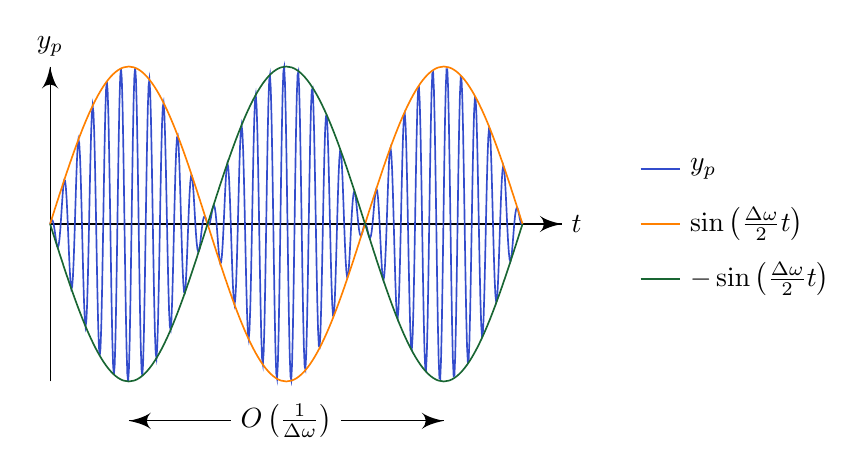
\begin{tikzpicture}
    \draw [->] (0, 0) -- (6.5, 0) node [right] {$t$};
    \draw [->] (0, -2) -- (0, 2) node [above] {$y_p$};

    \draw [semithick, mblue, domain=0:6,samples=600] plot(\x, {2 * cos(2000 * \x) * sin (90 * \x)});
    \draw [semithick, morange] (0, 0) sin (1, 2) cos (2, 0) sin (3, -2) cos (4, 0) sin (5, 2) cos (6, 0);
    \draw [semithick, mgreen] (0, 0) sin (1, -2) cos (2, 0) sin (3, 2) cos (4, 0) sin (5, -2) cos (6, 0);

    \draw [semithick, mblue] (7.5, 0.7) -- (8, 0.7) node [black, right] {$y_p$};
    \draw [semithick, morange] (7.5, 0) -- (8, 0) node [black, right] {$\sin\left(\frac{\Delta \omega}{2} t\right)$};
    \draw [semithick, mgreen] (7.5, -0.7) -- (8, -0.7) node [black, right] {$-\sin\left(\frac{\Delta \omega}{2} t\right)$};

    \draw [<->] (1, -2.5) -- (5, -2.5) node [pos=0.5,fill=white] {$O\left(\frac{1}{\Delta \omega}\right)$};
  \end{tikzpicture}
\end{center}
This oscillation in the amplitude of the $\cos$ wave is known as \emph{beating}. This happens when the forcing frequency is close to the natural frequency. The wavelength of the $\sin$ function has order $O(\frac{1}{\Delta \omega})$ and $\cos$ has wavelength $O(\frac{1}{\omega_0})$. As $\Delta\omega\to 0$, the wavelength of the beating envelope $\to \infty$ and we just have the initial linear growth.

Mathematically, since $\sin\theta \approx \theta$ as $\theta \to 0$, as $\Delta\omega \to 0$, we have
\[
  y_p\to \frac{-t}{2\omega_0}\cos\omega_0 t.
\]
In general, if the forcing is a linear combination of complementary functions, then the particular integral is proportional to $t$ (the independent variable) times the non-resonant guess.

\subsubsection{Variation of parameters}
So far, we have been finding particular integrals by guessing. Here we are going to come up with a method that can systematically help us find the particular integral. Of course, this is substantially more complicated than guessing. So if the form of the particular integral is obvious, we should go for guessing.

Let $y_1(x)$ and $y_2(x)$ be linearly independent complementary functions of the ODE $y'' + p(x)y' + q(x)y = f(x)$. Then the solution vectors $\mathbf{Y}_1 = (y_1, y_1')$ and $\mathbf{Y}_2 = (y_2, y_2')$ form a basis of the solution space. Note that theoretically, $\mathbf{Y}_1 = (0, 1)$ and $\mathbf{Y}_2 = (1, 0)$ also forms an equally valid basis, but this particular basis we've picked is the most helpful basis.

We can write
\[
  \mathbf{Y}_p(x) = u(x)\mathbf{Y}_1(x) + v(x)\mathbf{Y}_2(x).
\]
Component-wise, we have
\begin{align*}
  y_p &= uy_1 + vy_2 \tag{a}\\
  y_p' &= uy_1' + vy_2' \tag{b}
\end{align*}
Differentiating the second equation, we obtain
\[
  y''_p  = (uy_1'' + u'y_1') + (vy_2'' + v'y_2') \tag{c}
\]
If we use consider (c) + $p$(b) + $q$(a), we have $y_1' u' + y_2'v' = f$.

Now note that we derived the equation of $y_p'$ from the vector equation. This must be equal to what we get if we differentiate (a). By (a)$'$ - (b), we obtain $y_1u' + y_2v' = 0$. Now we have two simultaneous equations for $u'$ and $v'$, which we should be able to solve.

We can, for example, write them in matrix form as
\[
  \begin{pmatrix}
    y_1 & y_2\\
    y_1' & y_2'
  \end{pmatrix}
  \begin{pmatrix}
    u'\\
    v'
  \end{pmatrix}
  =
  \begin{pmatrix}
    0\\
    f
  \end{pmatrix}
\]
Inverting the left matrix, we have
\[
  \begin{pmatrix}
    u'\\
    v'
  \end{pmatrix} = \frac{1}{W}
  \begin{pmatrix}
    y_2' & -y_2\\
    -y_1' & y_1
  \end{pmatrix}
  \begin{pmatrix}
    0\\f
  \end{pmatrix}
\]
So $u' = -\frac{y_2}{W}f$ and $v' = \frac{y_1}{W}f$.

\begin{eg}
  $y'' + 4y = \sin 2x$. We know that $y_1 = \sin 2x$ and $y_2 = \cos 2x$. $W = -2$. We write
  \[
    y_p = u\sin 2x + v\cos 2x.
  \]
  Using the formulae above, we obtain
  \[
    u' = \frac{\cos 2x\sin 2x}{2} = \frac{\sin 4x}{4},\;\;\; v' = \frac{-\sin^2 2x}{2} = \frac{\cos 4x - 1}{4}
  \]
  So
  \[
    u = -\frac{\cos 4x}{16}, \;\;\; v = \frac{\sin 4x}{16} - \frac{x}{4}
  \]
  Therefore
  \[
    y_p = \frac{1}{16}(-\cos 4x\sin 2x + \sin 4x\cos 2x - \frac{x}{4}\cos 2x) = \frac{1}{16}\sin 2x - \frac{x}{4}\cos 2x
  \]
  Note that $-\frac{1}{4}x\cos 2x$ is what we found previously by detuning, and $\frac{1}{16}\sin 2x$ is a complementary function, so the results agree.
\end{eg}

It is generally not a good idea to remember the exact formula for the results we've obtained above. Instead, whenever faced with such questions, you should be able to re-derive the results instead.

\subsection{Linear equidimensional equations}
Equidimensional equations are often called homogeneous equations, but this is confusing as it has the same name as those with no forcing term. So we prefer this name instead.

\begin{defi}[Equidimensional equation]
  An equation is \emph{equidimensional} if it has the form
  \[
    ax^2y'' + bxy' + cy = f(x),
  \]
  where $a, b, c$ are constants.
\end{defi}
To understand the name ``equidimensional'', suppose we are doing physics and variables have dimensions. Say $y$ has dimensions $L$ and $x$ has dimensions $T$. Then $y'$ has dimensions $LT^{-1}$ and $y''$ has dimensions $LT^{-2}$. So all terms $x^2 y''$, $xy'$ and $y$ have the same dimensions.

\subsubsection*{Solving by eigenfunctions}
Note that $y = x^k$ is an eigenfunction of $x\frac{\d}{\d x}$. We can try an eigenfunction $y = x^k$. We have $y' = kx^{k - 1}$ and thus $xy' = kx^k = ky$; and $y'' = k(k - 1)x^{k - 2}$ and $x^2y'' = k(k - 1)x^k$.

Substituting in, we have
\[
  ak(k - 1) + bk + c = 0,
\]
which we can solve, in general, to give two roots $k_1$ and $k_2$, and $y_c = Ax^{k_1} + Bx^{k_2}$.

\subsubsection*{Solving by substitution}
Alternatively, we can make a substitution $z = \ln x$. Then we can show that
\[
  a^2\frac{\d ^2 y}{d z^2} + (b - a)\frac{\d y}{\d z} + cy = f(e^z).
\]
This turns an equidimensional equation into an equation with constant coefficients. The characteristic equation for solutions in the form $y = e^{\lambda z}$ is of form $a^2\lambda^2 + (b - a)\lambda + c = 0$, which we can rearrange to become $a\lambda(\lambda - 1) + b\lambda + c = 0$. So $\lambda = k_1, k_2$.

Then the complementary function is $y_c = Ae^{k_1z} + Be^{k_2z} = Ax^{k_1} + Bx^{k_2}$.

\subsubsection*{Degenerate solutions}
If the roots of the characteristic equation are equal, then $y_c = \{e^{kz}, ze^{kz}\} = \{x^k, x^k\ln x\}$. Similarly, if there is a resonant forcing proportional to $x^{k_1}$ (or $x^{k_2}$), then there is a particular integral of the form $x^{k_1}\ln x$.

These results can be easily obtained by considering the substitution method of solving, and then applying our results from homogeneous linear equations with constant coefficients.

\subsection{Difference equations}
Consider an equation of the form
\[
  a y_{n + 2} + by_{n + 1} + cy_n = f_n.
\]
We can solve in a similar way to differential equations, by exploiting linearity and eigenfunctions.

We can think of the difference operator $D[y_n] = y_{n + 1}$. This has an eigenfunction $y_n = k^n$. We have $D[y_n] = D[k^n] = k^{n + 1} = k\cdot k^n = ky_n$.

To solve the difference equation, we first look for complementary functions satisfying
\[
  ay_{n + 2} + by_{n + 1} + cy_n = 0
\]
We try $y_n = k^n$ to obtain
\begin{align*}
  ak^{n + 2} + bk^{n + 1} + ck^n &= 0\\
  ak^2 + bk + c &= 0
\end{align*}
from which we can determine $k$. So the general complementary function is $y_n^c = Ak_1^n + Bk_2^n$ if $k_1 \not= k_2$. If they are equal, then $y_n^c = (A + Bn)k^n$.

To find the particular integral, we guess.
\begin{center}
  \begin{tabular}{cc}
    \toprule
    $f_n$ & $y_n^p$\\
    \midrule
    $k^n$ & $Ak^n$ if $k \not= k_1, k_2$\\
    $k_1^n$ & $nk_1^n$\\
    $n^p$ & $An^p + Bn^{p - 1} + \cdots + Cn + D$\\
    \bottomrule
  \end{tabular}
\end{center}

\begin{eg}[Fibonacci sequence]
  The Fibonacci sequence is defined by
  \[
    y_n = y_{n - 1} + y_{n - 2}
  \]
  with $y_0 = y_1 = 1$.

  We can write this as
  \[
    y_{n + 2} - y_{n + 1} - y_n = 0
  \]
  We try $y_n = k^n$. Then $k^2 - k - 1 = 0$. Then
  \begin{align*}
    k^2 - k - 1 &= 0\\
    k &= \frac{1 \pm \sqrt{5}}{2}
  \end{align*}
  We write $k = \varphi_1, \varphi_2$. Then $y_n = A\varphi_1^n + B\varphi_2^n$. Our initial conditions give
  \begin{align*}
    A + B &= 1\\
    A\varphi_1 + B\varphi_2 &= 1
  \end{align*}
  We get $\displaystyle A = \frac{\varphi_1}{\sqrt{5}}$ and $\displaystyle B = \frac{-\varphi_2}{\sqrt{5}}$. So
  \[
    y_n = \frac{\varphi_1^{n + 1} - \varphi_2^{n + 1}}{\sqrt{5}} = \frac{\varphi_1^{n + 1} - \left(\frac{-1}{\varphi_1}\right)^{n + 1}}{\sqrt{5}}
  \]
\end{eg}

\subsection{Transients and damping}
In many physical systems, there is some sort of restoring force and some damping, eg. car suspension system.

Consider a car of mass $M$ with a vertical force $F(t)$ acting on it (eg. mouse jumping on the car). We can consider the wheels to be springs ($F = kx$) with a ``shock absorber'' ($F = l\dot x$). Then the equation of motion can be given by
\[
  M\ddot x = F(t) - kx - l\dot x.
\]
So we have
\[
  \ddot x + \frac{l}{M}\dot x + \frac{k}{M}x = \frac{1}{M}F(t).
\]
Note that if we don't have the damping and the forcing, we end up with a simple harmonic motion with angular frequency $\sqrt{k/M}$. Write $t = \tau \sqrt{M/k}$, where $\tau$ is dimensionless. The timescale $\sqrt{M/k}$ is proportional to the period of the undamped, unforced system (or 1 over its natural frequency). Then we obtain
\[
  \ddot x + 2\kappa\dot x + x = f(\tau)
\]
where, $\dot x$ means $\frac{\d x}{d\tau}$, $\kappa = \frac{l}{2\sqrt{kM}}$ and $f = \frac{F}{k}$.

By this substitution, we are now left with only one parameter $\kappa$ instead of the original three ($M, l, k$).

We will consider different possible cases.

\subsubsection*{Free (natural) response \texorpdfstring{$f = 0$}{f = 0}}
\begin{align*}
  \ddot x + 2\kappa \dot x + x &= 0\\
  \intertext{We try $x = e^{\lambda \tau}$}
  \lambda^2 + 2\kappa\lambda + 1 &= 0\\
  \lambda &= -\kappa \pm \sqrt{\kappa^2 - 1}\\
  &= -\lambda_1, -\lambda_2
\end{align*}
where $\lambda_1$ and $\lambda_2$ have positive real parts.

\subsubsection*{Underdamping}
If $\kappa < 1$, we have $x = e^{-\kappa\tau}(A\sin \sqrt{1 - \kappa^2}\tau  +B\cos \sqrt{1 - \kappa^2}\tau)$.

The period is $\frac{2\pi}{\sqrt{1 - \kappa^2}}$ and its amplitude decays in a characteristic of $O(\frac{1}{\kappa})$. Note that the damping increases the period. As $\kappa \to 1$, the oscillation period $\to \infty$.
\begin{center}
  \begin{tikzpicture}
    \draw [->] (0, 0) -- (6, 0) node [right] {$\tau$};
    \draw [->] (0, -2) -- (0, 2) node [above] {$x$};

    \draw [semithick, mblue, domain = 0:5.8, samples=100] plot (\x, {1.8 * exp (-0.5 * \x) * sin (300 * \x + 40)});
  \end{tikzpicture}
\end{center}

\subsubsection*{Critically damping}
If $\kappa = 1$, then $x = (A + B\tau)e^{-\kappa\tau}$.

The rise time and decay time are both $O(\frac{1}{\kappa}) = O(1)$. So the dimensional rise and decay times are $O(\sqrt{M/k})$.
\begin{center}
  \begin{tikzpicture}
    \draw [->] (0, 0) -- (6, 0) node [right] {$\tau$};
    \draw [->] (0, -2) -- (0, 2) node [above] {$x$};

    \draw [semithick, mblue, domain = 0:5.8, samples=100] plot (\x, {(1 + 3 * \x) * exp (-\x)});
  \end{tikzpicture}
\end{center}

\subsubsection*{Overdamping}
If $\kappa > 1$, then $x = Ae^{-\lambda_1\tau} + Be^{-\lambda_2\tau}$ with $\lambda_1 < \lambda_2$. Then the decay time is $O(1/\lambda_1)$ and the rise time is $O(1/\lambda_2)$.
\begin{center}
  \begin{tikzpicture}
    \draw [->] (0, 0) -- (6, 0) node [right] {$\tau$};
    \draw [->] (0, -2) -- (0, 2) node [above] {$x$};

    \draw [semithick, mblue, domain = 0:5.8, samples=100] plot (\x, {2 * exp (-0.3 * \x) - exp(-2 * \x)});
  \end{tikzpicture}
\end{center}
Note that in all cases, it is possible to get a large initial increase in amplitude.

\subsubsection*{Forcing}
In a forced system, the complementary functions typically determine the short-time transient response, while the particular integral determines the long-time (asymptotic) response.
For example, if $f(\tau) = \sin\tau$, then we can guess $x_p = C\sin \tau + D\cos\tau$. In this case, it turns out that $x_p = -\frac{1}{2\kappa}\cos\tau$.

The general solution is thus $x = Ae^{-\lambda_1\tau} + Be^{-\lambda \tau} - \frac{1}{2\kappa}\cos\tau \sim -\frac{1}{2\kappa}\cos\tau$ as $\tau\to \infty$ since $\re (\lambda_{1, 2}) > 0$.

It is important to note that the forcing response is out of phase with the forcing.
\subsection{Impulses and point forces}
\subsubsection{Dirac delta function}
Consider a ball bouncing on the ground. When the ball hits the ground at some time $T$, it experiences a force from the ground for some short period of time. The force on the ball exerted by the ground in $F(t)$ is $0$ for most of the time, except during the short period $(T - \varepsilon, T + \varepsilon)$.

Often we don't know (or we don't wish to know) the details of $F(t)$ but we can note that it only acts for a short time of $O(\varepsilon)$ that is much shorter than the overall time $O(t_2 - t_1)$ of the system. It is convenient mathematically to imagine the force acting instantaneously at time $t = T$, ie. consider the limit $\varepsilon\to 0$.

Newton's second law gives $m\ddot x = F(t) - mg$. While we cannot solve it, we can integrate the equation from $T - \varepsilon$ to $T + \varepsilon$. So
\begin{align*}
  \int_{T - \varepsilon}^{T + \varepsilon} m\frac{\d ^2 x}{\d t^2}\;\d t &= \int_{T - \varepsilon}^{T + \varepsilon} F(t)\;\d t - \int_{T - \varepsilon}^{T + \varepsilon}\;\d t\\
  \left[ m\frac{\d x}{\d t}\right]^{T + \varepsilon}_{T - \varepsilon} &= I - 2\varepsilon mg\\
  \Delta p &= I - O(\varepsilon)
\end{align*}
Where $\Delta p$ is the change in momentum and the impulse $I = \int_{T - \varepsilon}^{T + \varepsilon} F(t) \;\d t$ is the area under the force curve. Note that the impulse $I$ is the only property of $F$ that influences the macroscopic behaviour of the system. If the contact time $2\varepsilon$ is small, we'll neglect it and write
\[
  \Delta p = I
\]
Assuming that $F$ only acts on a negligible amount of time $\varepsilon$, all that matters to us is its integral $I$, ie. the area under the force curve.

wlog, assume $T = 0$ for easier mathematical treatment. We can consider a family of functions $D(t; \varepsilon)$ such that
\begin{gather*}
  \lim_{\varepsilon\to 0} D(t; \varepsilon) = 0 \text{ for all }t \not= 0;\\
  \lim_{\varepsilon\to 0}\int_{-\infty}^\infty D(t; \varepsilon) \;\d t = 1.
\end{gather*}
So we can replace the force in our example by $ID(t; \varepsilon)$, and then take the limit as $\varepsilon \to 0$.

For example, we can choose
\[
  D(t; \varepsilon) = \frac{1}{\varepsilon\sqrt{\pi}}e^{-t^2/\varepsilon^2}
\]
\begin{center}
  \begin{tikzpicture}
    \draw [->] (-3, 0) -- (3.25, 0) node [right] {$t$};
    \draw [->, use as bounding box] (0, 0) -- (0, 4) node [above] {$D$};

    \draw [semithick, mblue, domain=-3:3, samples = 100] plot (\x, { 1.6 * exp( - \x * \x)});
    \draw [semithick, morange, domain=-3:3, samples = 100] plot (\x, { 3.2 * exp( - 4 * \x * \x)});

    \draw [mblue, semithick] (3.5, 2.25) -- (4, 2.25) node [right, black] {$\varepsilon = 1$};
    \draw [morange, semithick] (3.5, 1.75) -- (4, 1.75) node [right, black] {$\varepsilon = 0.5$};
  \end{tikzpicture}
\end{center}
This has height $O(1/\varepsilon)$ and width $O(\varepsilon)$.

It can be checked that this satisfies the properties listed above. Note that as $\varepsilon \to 0$, $D(0; \varepsilon)\to \infty$. Therefore $\displaystyle \lim_{\varepsilon\to 0} D(t; \varepsilon)$ does not exist.

\begin{defi}[Dirac delta function]
  The \emph{Dirac delta function} is defined by
  \[
    \delta(x) = \lim_{\varepsilon \to 0} D(x; \varepsilon)
  \]
  on the understanding that we can only use its integral properties. For example, when we write
  \[
    \int_{-\infty}^{\infty} g(x)\delta (x) \;\d x,
  \]
  we actually mean
  \[
    \lim_{\varepsilon \to 0} \int_{-\infty}^{\infty} g(x)D(x; \varepsilon)\;\d x.
  \]
  In fact, this is equal to $g(0)$.

  More generally, $\int_a^b g(x)\delta(x - c)\;\d x = g(c)$ if $c\in (a, b)$ and $0$ otherwise, provided $g$ is continuous at $x = c$.
\end{defi}

This gives a convenient way of representing and making calculations involving impulsive or point forces. For example, in the previous example, we can write
\[
  m\ddot x = -mg + I\delta(t - T).
\]

\begin{eg}
  $y'' - y = 3\delta(x - \frac{\pi}{2})$ with $y = 0$ at $x = 0, \pi$. Note that or function $y$ is split into two parts by $x = \frac{\pi}{2}$.

  First consider the region $0 \leq x < \frac{\pi}{2}$. Here the delta function is $0$, and we have $y'' - y = 0$ and $y = 0$ and $x = 0$. Then $y = Ce^x + De^{-x} = A\sinh x + B\cosh x$ and obtain $B = 0$ from the boundary condition.
  In the region $\frac{\pi}{2} < x \leq \pi$, we again obtain $y = C\sinh(\pi - x) + D\cosh (\pi - x)$ and (from the boundary condition), $D = 0$.

  When $x = \frac{\pi}{2}$, first insist that $y$ is continuous at $x = \frac{\pi}{2}$. So $A = C$. Then note that we have to solve
  \[
    y'' - y = 3\delta\left(x - \frac{\pi}{2}\right)
  \]
  But remember that the delta function makes sense only in an integral. So we integrate both sides from $\frac{\pi}{2}^-$ to$\frac{\pi}{2}^+$. Then we obtain
  \[
    [y']^{\frac{\pi}{2}^+}_{\frac{\pi}{2}^-} - \int_{\frac{\pi}{2}^-}^{\frac{\pi}{2}^+} y\;\d x= 3
  \]
  Since we assume that $y$ is well behaved, the second integral is 0. So we are left with
  \[
    [y']^{\frac{\pi}{2}^+}_{\frac{\pi}{2}^-} = 3
  \]
  So we have
  \begin{align*}
    -C\cosh \frac{\pi}{2} - A\cosh\frac{\pi}{2} &= 3\\
    A = C &= \frac{-3}{2\cosh \frac{\pi}{2}}
  \end{align*}
\end{eg}
Then we have
\[
  y =
  \begin{cases}
    \frac{-3\sinh x}{2\cosh \frac{\pi}{2}} & 0 \leq x < \frac{\pi}{2}\\
    \frac{-3\sinh(\pi - x)}{2\cosh \frac{\pi}{2}} & \frac{\pi}{2} < x \leq \pi
  \end{cases}
\]
\begin{center}
  \begin{tikzpicture}
    \draw [->] (0, 0) -- (7, 0) node [right] {$x$};

    \draw [->] (0, 0) -- (0, -3.5) node [below] {$y$};

    \draw [semithick, mblue, domain=0:1.5708] plot ({2 * \x}, {-1.3 * sinh (\x)});
    \draw [semithick, mblue, domain=1.5708:3.14159] plot ({2 * \x}, {-1.3 * sinh (pi - \x)});
  \end{tikzpicture}
\end{center}
Note that at $x = \frac{\pi}{2}$, our final function has continuous $y$, discontinuous $y'$ and infinite $y''$. In general, differentiating a function makes it \emph{less} continuous. This is why we insisted at first that $y$ has to be continuous. Otherwise, $y'$ would look like a delta function, and $y''$ would be something completely unrecognizable.

Hence the discontinuity is always addressed by the highest order derivative since differentiation increases the discontinuity.

\subsection{Heaviside step function}

\begin{defi}[Heaviside step function]
  Define the Heaviside step function as:
  \[
    H(x) = \int_{-\infty}^x \delta(t) \;\d t
  \]
  We have
  \[
    H(x) =\begin{cases} 0 & x < 0\\1 & x > 0\\\text{undefined} & x = 0\end{cases}
  \]
  \begin{center}
    \begin{tikzpicture}
      \draw [->] (-3, 0) -- (3, 0) node [right] {$x$};
      \draw [->] (0, 0) -- (0, 3) node [above] {$y$};

      \draw [mblue, semithick] (-3, 0) -- (0, 0);
      \draw [mblue, semithick] (0, 2) -- (3, 2);
    \end{tikzpicture}
  \end{center}
  By the fundamental theorem of calculus,
  \[
    \frac{\d H}{\d x} = \delta(x)
  \]
  But remember that these functions and relationships can only be used inside integrals.
\end{defi}

\section{Series solutions}
Often, it is difficult to solve a differential equation directly. However, we can attempt to find a Taylor series for the solution.

We will consider equations of the form
\[
  p(x) y'' + q(x) y' + r(x) y = 0.
\]
\begin{defi}[Ordinary and singular points]
  The point $x = x_0$ is an \emph{ordinary point} of the differential equation if $\frac{q}{p}$ and $\frac{r}{p}$ have Taylor series about $x_0$ (ie. are ``analytic'', cf. Complex Analysis). Otherwise, $x_0$ is a \emph{singular point}.

  If $x_0$ is a singular point but the equation can be written as
  \[
    P(x)(x - x_0)^2y'' + Q(x)(x - x_0)y' + R(x)y = 0,
  \]
  where $\frac{Q}{P}$ and $\frac{R}{P}$ have Taylor series about $x_0$, then $x_0$ is a \emph{regular singular point}.
\end{defi}

\begin{eg}\leavevmode
  \begin{enumerate}
    \item $(1 - x^2)y'' - 2cy' + 2y = 0$. $x = 0$ is an ordinary point. However, $x = \pm 1$ are (regular) singular points since $p(\pm 1) = 0$.
    \item $\sin x y'' + \cos x y' + 2y = 0$. $x = n\pi$ are regular singular points while all others are ordinary.
    \item $(1 + \sqrt{x}) y'' - 2xy' + 2y = 0$. $x = 0$ is an irregular singular point because $\sqrt{x}$ is not differentiable at $x = 0$.
  \end{enumerate}
\end{eg}

It is possible to show that if $x_0$ is an ordinary point, then the equation is guaranteed to have two linearly independent solutions of the form
\[
  y = \sum_{n = 0}^\infty a_n(x - x_0)^n,
\]
ie. Taylor series about $x_0$. The solution must be convergent in some neighbourhood of $x_0$.

If $x_0$ is a regular singular point, then there is at least one solution of the form
\[
  y = \sum_{n = 0}^\infty a_n(x - x_0)^{n + \sigma}
\]
with $a_0 \not= 0$ (to ensure $\sigma$ is unique). The \emph{index} $\sigma$ can be any complex number. This is called a Frobenius series.

Alternatively, it can be nice to think of the Frobenius series as
\begin{align*}
  y &= (x - x_0)^\sigma \sum_{n = 0}^\infty a_n (x - x_0)^n\\
  &= (x-x_0)^\sigma f(x)
\end{align*}
where $f(x)$ is analytic and has a Taylor series.

We will not prove these results, but merely apply them.

\subsubsection*{Ordinary points}
\begin{eg}
  Consider $(1 - x^2)y'' - 2xy' + 2y = 0$. Find a series solution about $x = 0$ (which is an ordinary point).

  We try $y = \sum_{n = 0}^\infty a_nx^n$. First, we write the equation in the form of an equidimensional equation with polynomial coefficients by multiplying both sides by $x^2$. This little trick will make subsequent calculations slightly nicer. We obtain
  \begin{align*}
    (1 - x)^2 (x^2y'') - 2x^2(xy') + 2x^2 y &= 0\\
    \sum a_n[(1 - x^2) n(n - 1) - 2x^2n + 2x^2]x^n &= 0\\
    \sum a_n[n(n - 1) + (-n^2 - n + 2)x^2]x^n &= 0
  \end{align*}
  We look at the coefficient of $x^n$ and obtain the following general recurrence relation:
  \begin{gather*}
    n(n - 1) a_n + [-(n - 2)^2 - (n - 2) + 2]a_{n - 2} = 0\\
    n(n - 1)a_n = (n^2 - 3n)a_{n - 2}
  \end{gather*}
  Here we do \emph{not} divide by anything since they might be zero.

  First consider the case $n = 0$. The left hand side gives $0\cdot a_0 = 0$ (the right hand side is $0$ since $a_{n - 2} = 0$). So any value of $a_0$ satisfies the recurrence relationship, and it can take any arbitrary value. This corresponds to a constant of integration. Similarly, by considering $n = 1$, $a_1$ is arbitrary.

  For $n > 1$, $n$ and $n - 1$ are non-zero. So we have
  \begin{align*}
    a_n &= \frac{n - 3}{n - 1} a_{n - 2}\\
    \intertext{In this case (but generally not), we can further simplify it to obtain:}
    a_n &= \frac{n - 3}{n - 1}\frac{n - 5}{n - 3}a_{n - 4}\\
    &= \frac{n - 5}{n - 1}a_{n - 4}\\
    &\;\;\vdots
    \intertext{So}
    a_{2k} &= \frac{-1}{2k - 1}a_0,\\
    a_{2k + 1} &= 0.
  \end{align*}
  So we obtain
  \begin{align*}
    y &= a_0[1 - \frac{x^2}{1} - \frac{x^4}{3} - \frac{x^6}{5} - \cdots] + a_1 x\\
    &= a_0\left[1 - \frac{x}{2}\ln\left(\frac{1 + x}{1 - x}\right)\right] + a_1x
  \end{align*}
  Notice the logarithmic behaviour near $x = \pm 1$ which are regular singular points.
\end{eg}

\subsubsection*{Regular singular points}
\begin{eg}
  Consider $4xy'' + 2(1 - x^2)y' - xy = 0$. Note that $x = 0$ is a singular point. However, if we multiply throughout by $x$ to obtain an equidimensional equation, we obtain
  \[
    4(x^2 y'') + 2(1 - x^2)xy' - x^2 y = 0.
  \]
  Since $\frac{Q}{P} = \frac{1 - x^2}{2}$ and $\frac{R}{P} = \frac{x^2}{4}$ both have Taylor series, $x = 0$ is a regular singular point. Try
  \[
    y = \sum_{n = 0}^\infty a_n x^{n + \sigma}\text{ with }a_0 \not= 0.
  \]
  Substituting in, we have
  \[
    \sum a_n x^{n + \sigma}[4(n + \sigma)(n + \sigma - 1) + 2(1 - x^2)(n + \sigma) - x^2]
  \]
  By considering the coefficient of $x^{n + \sigma}$, we obtain the general recurrence relation
  \[
    [4(n + \sigma)(n + \sigma - 1) + 2(n + \sigma)]a_n -[2(n - 2 + \sigma) + 1]a_{n - 2} = 0.
  \]
  Simplifying the equation gives
  \[
    2(n + \sigma)(2n + 2\sigma - 1)a_n = (2n + 2\sigma-3)a_{n - 2}.
  \]
  The $n = 0$ case gives the \emph{indicial equation} for the \emph{index} $\sigma$:
  \[
    2\sigma(2\sigma - 1)a_0 = 0.
  \]
  Since $a_0 \not= 0$, we must have $\sigma = 0$ or $\frac{1}{2}$. The $\sigma = 0$ solution corresponds to an analytic (``Taylor series'') solution, while $\sigma = \frac{1}{2}$ corresponds to a non-analytic one.

  When $\sigma = 0$, the recurrence relation becomes
  \[
    2n(2n - 1)a_n = (2n - 3)a_{n - 2}.
  \]
  When $n = 0$, this gives $0\cdot a_0 = 0$. So $a_0$ is arbitrary. For $n >0$, we can divide and obtain
  \[
    a_n = \frac{2n - 3}{2n(2n - 1)}a_{n - 2}.
  \]
  We can see that $a_1 = 0$ and so are subsequent odd terms.

  If $n = 2k$, ie. is even, then
  \begin{align*}
    a_{2k} &= \frac{4k - 3}{4k(4k - 1)}a_{2k - 2}\\
    y &= a_0\left[1 + \frac{1}{4\cdot 3}x^2 + \frac{5}{8\cdot 7\cdot 4\cdot 3}x^4 + \cdots\right]
  \end{align*}
  Note that we have only found one solution in this case.

  Now when $\sigma = \frac{1}{2}$, we obtain
  \[
    (2n + 1)(2n)a_n = (2n - 2)a_{n - 2}
  \]
  When $n = 0$, we obtain $0\cdot a_0 = 0$, so $a_0$ is arbitrary. To avoid confusion with the $a_0$ above, call it $b_0$ instead.

  When $n = 1$, we obtain $6a_1 = 0$ and $a_1 = 0$ and so are subsequent odd terms.

  For even $n$,
  \[
    a_n = \frac{n - 1}{n(2n + 1)}a_{n - 2}
  \]
  So
  \[
    y = b_0 x^{1/2}\left[1 + \frac{1}{2\cdot 5}x^2 + \frac{3}{2\cdot 5\cdot 4\cdot 9}x^4 + \cdots\right]
  \]
\end{eg}

\subsubsection*{Resonance of solutions}
Note that the indicial equation has two roots $\sigma_1, \sigma_2$. Consider the two different cases:
\begin{enumerate}
  \item If $\sigma_2 - \sigma_1$ is not an integer, then there are two linearly independent Frobenius solutions
    \[
      y = \left[(x - x_0)^{\sigma_1}\sum_{n = 0}^{\infty} a_n(x - x_0)^n\right] + \left[(x - x_0)^{\sigma_2}\sum_{n = 0}^{\infty} b_n(x - x_0)^n\right].
    \]
    As $x\to x_0$, $y \sim (x - x_0)^{\sigma_1}$, where $\re(\sigma_1) \leq \re(\sigma_2)$

  \item If $\sigma_2 - \sigma_1$ is an integer (including when they are equal), there is one solution of the form
    \[
      y_1 = (x - x_0)^{\sigma_2}\sum_{n = 0}^{\infty} a_n(x - x_0)^n
    \]
    with $\sigma_2 \geq \sigma_1$.

    In this case, $\sigma = \sigma_1$ will not give a valid solution, as we will later see. Instead, the other solution is (usually) in the form
    \[
      y_2 = \ln(x - x_0)y_1 + \sum_{n = 0}^\infty b_n(x - x_0)^n.
    \]
    This form arises from resonance between the two solutions. But if the resonance somehow avoids itself, we can possibly end up with two regular Frobenius series solutions.

    We can substitute this form of solution into the differential equation to determine $b_n$.
\end{enumerate}
\begin{eg}
  Consider $x^2 y'' - xy = 0$. $x = 0$ is a regular singular point. It is already in equidimensional form $(x^2y'') - x(y) = 0$. Try
  \[
    y = \sum_{n = 0}^\infty a_n x^n
  \]
  with $a_0 \not= 0$. We obtain
  \[
    \sum a_nx^{n + \sigma}[(n + \sigma)(n + \sigma - 1) - x] = 0.
  \]
  The general recurrence relation is
  \[
    (n + \sigma)(n + \sigma - 1)a_n = a_{n - 1}.
  \]
  $n = 0$ gives the indicial equation
  \[
    \sigma(\sigma - 1) = 0.
  \]
  Then $\sigma = 0, 1$. We are guaranteed to have a solution in the form $\sigma = 1$. When $\sigma = 1$, the recurrence relation becomes
  \[
    (n + 1)n a_n = a_{n - 1}.
  \]
  When $n = 0$, $0\cdot a_0 = 0$ so $a_0$ is arbitrary.
  When $n > 0$, we obtain
  \[
    a_n = \frac{1}{n(n +1)}a_{n - 1} = \frac{1}{(n + 1)(n!)^2}a_0.
  \]
  So
  \[
    y_1 = a_0x\left(1 + \frac{x}{2} + \frac{x^2}{12} + \frac{x^3}{144} + \cdots \right).
  \]
  When $\sigma = 0$, we obtain
  \[
    n(n - 1)a_n = a_{n - 1}.
  \]
  When $n = 0$, $0\cdot a_0 = 0$ and $a_0$ is arbitrary. When $n = 1$, $0\cdot a_1 = a_0$. However, $a_0\not= 0$ by our initial constraint. Contradiction. So there is no solution in this form (If we ignore the constraint that $a_0\not= 0$, we know that $a_0$ is arbitrary. But this gives exactly the same solution we found previously with $\sigma = 1$)

  The other solution is thus in the form
  \[
    y_2 = y_1\ln x + \sum_{n = 0}^\infty b_nx^n.
  \]
\end{eg}
\section{Directional derivative}
\label{sec:directional-derivative}
\subsection{Gradient vector}
Consider a function $f(x, y)$ and a displacement $\d\mathbf{s} = (\d x, \d y)$. The change in $f(x, y)$ during that displacement is
\[
  \d f = \frac{\partial f}{\partial x}\d x + \frac{\partial f}{\partial y}\d y
\]
We can also write this as
\begin{align*}
  \d f &= (\d x, \d y)\cdot \left(\frac{\partial f}{\partial x}, \frac{\partial f}{\partial y}\right)\\
  &= \d\mathbf{s}\cdot \nabla f
\end{align*}
where $\nabla f = \mathrm{grad}f = \left(\frac{\partial f}{\partial x}, \frac{\partial f}{\partial y}\right)$ are the Cartesian components of the \emph{gradient} of $f$.

We write $\d\mathbf{s} = \hat{\mathbf{s}}\;\d s$, where $|\hat{\mathbf{s}}| = 1$. Then
\begin{defi}[Directional derivative]
  The \emph{directional derivative} of $f$ in the direction of $\hat{\mathbf{s}}$ is
  \[
    \frac{\d f}{\d s} = \hat{\mathbf{s}}\cdot \nabla f.
  \]
\end{defi}

\begin{defi}[Gradient vector]
  The \emph{gradient vector} $\nabla f$ is defined as the vector that satisfies
  \[
    \frac{\d f}{\d s} = \mathbf{\hat{s}}\cdot \nabla f.
  \]
\end{defi}
Officially, we take this to be the definition of $\nabla f$. Then $\nabla f = \left(\frac{\partial f}{\partial x}, \frac{\partial f}{\partial y}\right)$ is a theorem that can be proved from this definition.

We know that the directional derivative is given by
\[
  \frac{\d f}{\d s} = \mathbf{\hat{s}}\cdot \nabla f = |\nabla f| \cos \theta
\]
where $\theta$ is the angle between the displacement and $\nabla f$. Then when $\cos\theta$ is maximized, $\frac{\d f}{\d s} = |\nabla f|$. So we know that
\begin{enumerate}
  \item $\nabla f$ has magnitude equal to the maximum rate of change of $f(x, y)$ in the $xy$ plane.
  \item It has direction in which $f$ increases most rapidly.
  \item If $\d\mathbf{s}$ is a displacement along a contour of $f$ (ie. along a line in which $f$ is constant), then
    \[
      \frac{\d f}{\d s} = 0.
    \]
    So $\mathbf{\hat{s}}\cdot \nabla f = 0$, ie. $\nabla f$ is orthogonal to the contour.
\end{enumerate}
\subsection{Stationary points}
There is always (at least) one direction in which $\frac{\d f}{\d s} = 0$, namely the direction parallel to the contour of $f$. However, local maxima and minima have
\[
  \frac{\d f}{\d s} = 0
\]
for \emph{all} directions, ie. $\mathbf{\hat{s}}\cdot \nabla f = 0$ for all $\mathbf{\hat{s}}$, ie. $\nabla f = \mathbf{0}$. Then we know that
\[
  \frac{\partial f}{\partial x} = \frac{\partial f}{\partial y} = 0.
\]
However, apart from maxima and minima, in 3 dimensions, we also have saddle points:
\begin{center}
  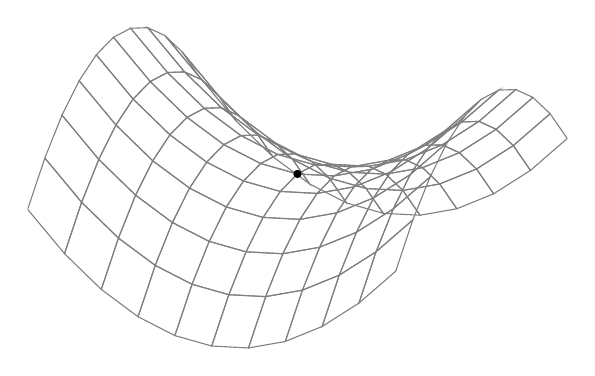
\begin{tikzpicture}
    \begin{axis}[hide axis, xtick=\empty, ytick=\empty]
      \addplot3 [mesh, draw=gray, samples = 11] {x^2 - y^2};
      \node [circ] at (axis cs:0, 0, 0) {};
    \end{axis}
  \end{tikzpicture}
\end{center}
In general, we define a saddle point to be a point at which $\nabla f = 0$ but is not a maximum or minimum.

When we plot out contours of functions, near maxima and minima, the contours are locally elliptical. Near saddle points, they are locally hyperbolic. Also, the contour lines cross at and only at saddle points.

\subsection{Taylor series for multi-variable functions}
Suppose we have a function $f(x, y)$ and a point $\mathbf{x}_0$. Now consider a finite displacement $\delta s$ along a straight line in the $x,y$ plane. Then
\[
  \delta s\frac{\d }{\d s} = \delta \mathbf{s}\cdot \nabla
\]
The Taylor series along the line is
\begin{align*}
  f(s) &= f(s_0 + \delta s)\\
  &=f(s_0) + \delta s\frac{\d f}{\d s} + \frac{1}{2}(\delta s)^2\frac{\d ^2 f}{\d s^2}\\
  &= f(s_0) + \delta \mathbf{s} \cdot \nabla f + \frac{1}{2}\delta s^2 (\mathbf{\hat{s}}\cdot \nabla)(\mathbf{\hat{s}}\cdot \nabla)f.
\end{align*}
We get
\begin{align*}
  \delta \mathbf{s}\cdot \nabla f &= (\delta x)\frac{\partial f}{\partial x} + (\delta y)\frac{\partial f}{\partial y}\\
  &= (x - x_0)\frac{\partial f}{\partial x} + (y - y_0)\frac{\partial f}{\partial y}
\end{align*}
and
\begin{align*}
  \delta s^2 (\mathbf{\hat{s}}\cdot \nabla)(\mathbf{\hat{s}}\cdot \nabla)f &= (\delta \mathbf{s}\cdot \nabla)(\delta \mathbf{s}\cdot \nabla) f\\
  &= \left[\delta x\frac{\partial }{\partial x} + \delta y\frac{\partial}{\partial y}\right]\left[\delta x\frac{\partial f}{\partial x} + \delta y\frac{\partial f}{\partial y}\right]\\
  &= \delta x^2 \frac{\partial^2 f}{\partial x^2} + 2\delta x\delta y\frac{\partial^2 f}{\partial x\partial y} + \delta y^2 \frac{\partial^2 f}{\partial y^2}\\
  &=
  \begin{pmatrix}
    \delta x& \delta y
  \end{pmatrix}
  \begin{pmatrix}
    f_{xx}&f_{xy}\\
    f_{yx}&f_{yy}
  \end{pmatrix}
  \begin{pmatrix}
    \delta x\\\delta y
  \end{pmatrix}
\end{align*}
\begin{defi}[Hessian matrix]
  The \emph{Hessian matrix} is the matrix
  \[
    \nabla \nabla f =
    \begin{pmatrix}
      f_{xx}&f_{xy}\\
      f_{yx}&f_{yy}
    \end{pmatrix}
  \]
\end{defi}

In conclusion, we have
\begin{align*}
  f(x, y) &= f(x_0, y_0) + (x - x_0)f_x + (y - y_0)f_y \\
  &+ \frac{1}{2}[(x - x_0)^2 f_{xx} + 2(x - x_0)(y - y_0)f_{xy} + (y - y_0)^2 f_yy]
\end{align*}
In general, the coordinate-free form is
\[
  f(\mathbf{x}) = f(\mathbf{x_0}) + \delta \mathbf{x}\cdot\nabla f(\mathbf{x}_0) + \frac{1}{2}\delta \mathbf{x}\cdot \nabla \nabla f\cdot \delta \mathbf{x}
\]
where the dot in the second term represents a matrix product. Alternatively, in terms of the gradient operator (and real dot products), we have
\[
  f(\mathbf{x}) = f(\mathbf{x_0}) + \delta \mathbf{x}\cdot \nabla f(\mathbf{x}_0) + \frac{1}{2}[\nabla (\nabla f\cdot \delta \mathbf{x})]\cdot \delta\mathbf{x}
\]

\subsection{Classification of stationary points}
At a stationary point $\mathbf{x}_0$, we know that $\nabla f(\mathbf{x}_0) = 0$. So at a point near the stationary point,
\[
  f(\mathbf{x})\approx f(\mathbf{x}_0) + \frac{1}{2}\delta\mathbf{x}\cdot H\cdot \delta\mathbf{x},
\]
where $H = \nabla\nabla f(\mathbf{x}_0)$  is the Hessian matrix.

At a minimum, Every point near $\mathbf{x}_0$ has $f(\mathbf{x}) > f(\mathbf{x}_0)$, ie. $\delta \mathbf{x}\cdot H\cdot \delta \mathbf{x} > 0$ for all $\delta \mathbf{x}$. We say $\delta \mathbf{x}\cdot H\cdot\delta \mathbf{x}$ is \emph{positive definite}.

Similarly, at a maximum, $\delta \mathbf{x}\cdot H\cdot \delta\mathbf{x} < 0$ for all $\delta \mathbf{x}$. We say $\delta \mathbf{x}\cdot H\cdot \delta \mathbf{x}$ is \emph{negative definite}.

At a saddle, $\delta \mathbf{x} \cdot H\cdot \delta\mathbf{x}$ is indefinite, ie. it can be positive, negative or zero depending on the direction.

This, so far, is not helpful, since we do not have an easy way to know what sign $\delta \mathbf{x}\cdot H\cdot \delta \mathbf{x}$ could be. Now note that $H = \nabla\nabla f$ is symmetric (because $f_{xy} = f_{yx}$). So $H$ can be diagonalized (cf. Vectors and Matrices). With respect to these axes in which $H$ is diagonal (principal axes), we have
\begin{align*}
  \delta\mathbf{x}\cdot H\cdot \delta\mathbf{x} &= (\delta x, \delta y, \cdots, \delta z)
  \begin{pmatrix}
    \lambda_1\\
    &\lambda_2\\
    &&\ddots\\
    &&&\lambda_n
  \end{pmatrix}
  \begin{pmatrix}
    \delta x\\\delta y\\\vdots\\\delta z
  \end{pmatrix}\\
  &= \lambda_1(\delta x)^2 + \lambda_2 (\delta y)^2 + \cdots + \lambda_n(\delta z)^2
\end{align*}
where $\lambda_1, \lambda_2, \cdots \lambda_n$ are the eigenvalues of $H$.

So for $\delta \mathbf{x}\cdot H\cdot \delta \mathbf{x}$ to be positive-definite, we need $\lambda_i > 0$ for all $i$. Similarly, it is negative-definite iff $\lambda_i < 0$ for all $i$. If eigenvalues have mixed sign, then it is a saddle point.

Finally, if there is at least one zero eigenvalue, then we need further analysis to determine the nature of the stationary point.

Apart from finding eigenvalues, another way to determine the definiteness is using the \emph{signature}.
\begin{defi}[Signature of Hessian matrix]
  The \emph{signature} of $H$ is the pattern of the signs of the subdeterminants:
  \[
    \underbrace{f_{xx}}_{|H_1|},
    \underbrace{
      \begin{vmatrix}
        f_{xx} & f_{xy}\\
        f_{yx} & f_{yy}
      \end{vmatrix}}_{|H_2|},\cdots,
    \underbrace{\begin{vmatrix}
      f_{xx} & f_{xy} & \cdots & f_{xz}\\
      f_{yx} & f_{yy} & \cdots & f_{yz}\\
      \vdots & \vdots & \ddots & \vdots\\
      f_{zx} & f_{zy} & \cdots & f_{zz}
    \end{vmatrix}}_{|H_n| = |H|}
  \]
\end{defi}

\begin{prop}
  $H$ is positive definite if and only if the signature is $+, +, \cdots, +$. $H$ is negative definite if and only if the signature is $-, +, \cdots, (-1)^n$. Otherwise, $H$ is indefinite.
\end{prop}

\subsection{Contours of \texorpdfstring{$f(x, y)$}{f(x, y)}}
Consider $H$ in 2 dimensions, and axes in which $H$ is diagonal. So $H =
\begin{pmatrix}
  \lambda_1 & 0\\
  0 & \lambda_2
\end{pmatrix}$. Write $\mathbf{x} - \mathbf{x}_0 = (X, Y)$.

Then near $\mathbf{x}_0$, $f = $ constant $\Rightarrow \mathbf{x}H\mathbf{x} = $ constant, ie. $\lambda_1 X^2 + \lambda_2 Y^2 = $ constant. At a maximum or minimum, $\lambda_1$ and $\lambda_2$ have the same sign. So these contours are locally ellipses. At a saddle point, they have different signs and the contours are locally hyperbolae.

\begin{eg}
  Find and classify the stationary points of $f(x, y) = 4x^3 - 12xy + y^2 + 10y + 6$. We have
  \begin{align*}
    f_x &= 12x^2 - 12y\\
    f_y &= -12x + 2y + 10\\
    f_{xx} &= 24x\\
    f_{xy} &= -12\\
    f_{yy} &= 2
  \end{align*}
  At stationary points, $f_x = f_y = 0$. So we have
  \[
    12x^2 - 12y = 0,\quad -12x + 2y + 10 = 0.
  \]
  The first equation gives $y = x^2$. Substituting into the second equation, we obtain $x = 1, 5$ and $y = 1, 25$ respectively. So the stationary points are $(1, 1)$ and $(5, 25)$

  To classify them, first consider $(1, 1)$. Our Hessian matrix $H =
  \begin{pmatrix}
    24 & -12\\
    -12 & 2
  \end{pmatrix}$. Our signature is $|H_1| = 24$ and $|H_2| = -96$. Since we have a $+, -$ signature, this an indefinite case and it is a saddle point.

  At $(5, 25)$, $H =
  \begin{pmatrix}
    120 & -12\\
    -12 & 2
  \end{pmatrix}$
  So $|H_1| = 120$ and $|H_2| = 240 - 144 = 96$. Since the signature is $+, +$, it is a minimum.

  To draw the contours, we draw what the contours look like near the stationary points, and then try to join them together, noting that contours cross only at saddles.
  \begin{center}
    \includegraphics[width=300pt]{images/de_contour.pdf}
  \end{center}
\end{eg}

\section{Systems of differential equations}
\subsection{Linear equations}
Consider two dependent variables $y_1(t), y_2(t)$ related by
\begin{align*}
  \dot y_1 &= ay_1 + by_2 + f_1(t)\\
  \dot y_2 &= cy_1 + dy_2 + f_2(t)
\end{align*}
We can write this in vector notation by
\[
  \begin{pmatrix}
    \dot y_1\\\dot y_2
  \end{pmatrix} =
  \begin{pmatrix}
    a & b\\
    c & d
  \end{pmatrix}
  \begin{pmatrix}
    y_1\\y_2
  \end{pmatrix}
  \begin{pmatrix}
    f_1\\f_2
  \end{pmatrix}
\]
or $\mathbf{\dot Y} = M\mathbf{Y} + \mathbf{F}$. We can convert this to a higher-order equation by
\begin{align*}
  \ddot y_1 &= a\dot y_1 + b\dot y_2 + \dot f_1\\
  &= a\dot y_1 + b(cy_1 + dy_2 + f_2) + \dot f_1\\
  &= a\dot y_1 + bcy_1 + d(\dot y_1 - ay_1 - f_1) + bf_2 + \dot f_1
\end{align*}
so
\[
  \ddot y_1 - (a + d)\dot y_1 + (ad - bc) y_1 = bf_2 - df_1 + \dot f_1
\]
and we know how to solve this. However, this actually complicates the equation.

So what we usually do is the other way round: if we have a high-order equation, we can do this to change it to a system of first-order equations:

If $\ddot y + a\dot y + by = f$, write $y_1 = y$ and $y_2 = \dot y$. Then let $\mathbf{Y} =
\begin{pmatrix}
  y\\\dot y
\end{pmatrix}$

Our system of equations becomes
\begin{align*}
  \dot y_1 &= y_2\\
  \dot y_2 &= f - a y_2 - by_1
\end{align*}
or
\[
  \mathbf{\dot{Y}} =
  \begin{pmatrix}
    0 & 1\\
    -b & -a
  \end{pmatrix}
  \begin{pmatrix}
    y_1\\y_2
  \end{pmatrix}
  \begin{pmatrix}
    0 \\ f
  \end{pmatrix}.
\]
Now consider the general equation
\begin{align*}
  \mathbf{\dot {Y}} &= M\mathbf{Y} + \mathbf{F}\\
  \mathbf{\dot {Y}} - M\mathbf{Y} &= \mathbf{F}
\end{align*}
We first look for a complementary solution $\mathbf{Y}_c = \mathbf{v} e^{\lambda t}$, where $\mathbf{v}$ is a constant vector. So we get
\[
  \lambda\mathbf{v} - M\mathbf{v} = \mathbf{0}.
\]
We can write this as
\[
  M\mathbf{v} = \lambda \mathbf{v}.
\]
So $\lambda$ is the eigenvalue of $M$ and $\mathbf{v}$ is the corresponding eigenvector.

We can solve this by solving the characteristic equation $\det(M - \lambda I) = 0$. Then for each $\lambda$, we find the corresponding $\mathbf{v}$.

\begin{eg}
  \[
    \mathbf{\dot{Y}} =
    \begin{pmatrix}
      -4 & 24\\
      1 & -2
    \end{pmatrix}
    \mathbf{Y} =
    \begin{pmatrix}
      4\\1
    \end{pmatrix}e^t
  \]
  The characteristic equation of $M$ is $
  \begin{vmatrix}
    -4 - \lambda & 24\\
    1 & -2 - \lambda
  \end{vmatrix} = 0$, which gives $(\lambda + 8)(\lambda - 2) = 0$ and $\lambda = 2, -8$.

  When $\lambda = 2$, $\mathbf{v}$ satisfies
  \[
    \begin{pmatrix}
      -6 & 24\\
      1 & -4
    \end{pmatrix}
    \begin{pmatrix}
      v_1\\v_2
    \end{pmatrix} = \mathbf{0},
  \]
  and we obtain $\mathbf{v}_1 =
  \begin{pmatrix}
    4\\1
  \end{pmatrix}$.

  When $\lambda = -8$, we have
  \[
    \begin{pmatrix}
      4 & 24\\
      1 & 6
    \end{pmatrix}
    \begin{pmatrix}
      v_1\\v_2
    \end{pmatrix} = \mathbf{0},
  \]
  and $\mathbf{v}_2 =
  \begin{pmatrix}
    -6 \\1
  \end{pmatrix}$. So the complementary solution is
  \[
    \mathbf{Y} = A
    \begin{pmatrix}
      4\\1
    \end{pmatrix}e^{2t} + B
    \begin{pmatrix}
      -6\\1
    \end{pmatrix}e^{-8t}
  \]
  To plot the phase-space trajectories, we first consider the cases where $\mathbf{Y}$ is an eigenvector.  If $\mathbf{Y}$ is an integer multiple of $\begin{pmatrix}4\\1\end{pmatrix}$, then it will keep moving outwards in the same direction. Similarly, if it is an integer multiple of $\begin{pmatrix}-6\\1\end{pmatrix}$, it will move towards the origin.
  \begin{center}
    \begin{tikzpicture}
      \draw [->] (-4, 0) -- (4, 0) node [right] {$y_1$};
      \draw [->] (0, -2) -- (0, 2) node [above] {$y_2$};

      \draw [->-=0.785, -<-=0.215, mblue, semithick] (-4, -1) -- (4, 1) node [right] {$v_1 = (4, 1)$};
      \draw [->-=0.25, -<-=0.75, mblue, semithick] (-4, 0.667) -- (4, -0.667) node [right] {$v_2 = (-6, 1)$};
    \end{tikzpicture}
  \end{center}
  We can now add more (curved) lines based on these two:
  \begin{center}
    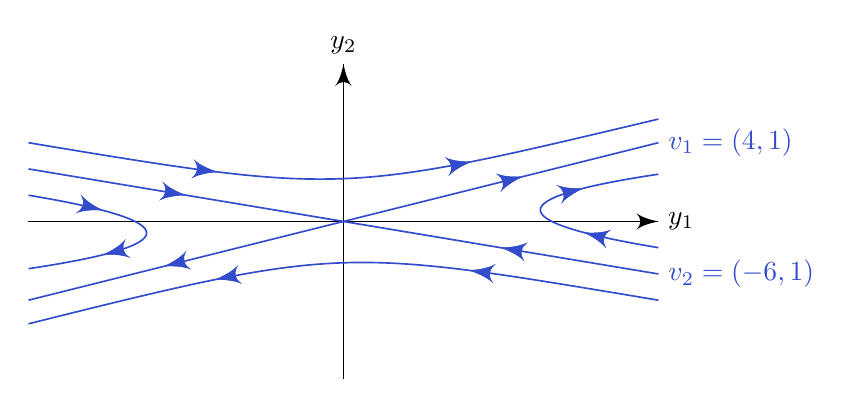
\begin{tikzpicture}
      \draw [->] (-4, 0) -- (4, 0) node [right] {$y_1$};
      \draw [->] (0, -2) -- (0, 2) node [above] {$y_2$};

      \draw [->-=0.785, -<-=0.215, mblue, semithick] (-4, -1) -- (4, 1) node [right] {$v_1 = (4, 1)$};
      \draw [->-=0.25, -<-=0.75, mblue, semithick] (-4, 0.667) -- (4, -0.667) node [right] {$v_2 = (-6, 1)$};

      \draw [mblue, semithick, ->- = 0.3, ->- = 0.7] (-4, 1) .. controls (0, 0.333) and (0, 0.35) .. (4, 1.3);
      \draw [mblue, semithick, -<- = 0.3, -<- = 0.7] (-4, -1.3) .. controls (0, -0.3) and (0, -0.333) .. (4, -1);

      \draw [mblue, semithick, ->- = 0.3, ->- = 0.7] (-4, 0.333) .. controls (-2, 0) and (-2, -0.3) .. (-4, -0.6);
      \draw [mblue, semithick, ->- = 0.3, ->- = 0.7] (4, -0.333) .. controls (2, 0) and (2, 0.3) .. (4, 0.6);
    \end{tikzpicture}
  \end{center}
  To find the particular integral, we try $\mathbf{Y}_p = \mathbf{u}e^t$. Then
  \begin{align*}
    \begin{pmatrix}
      u_1\\u_2
    \end{pmatrix} -
    \begin{pmatrix}
      -4 & 24\\
      1 & -2
    \end{pmatrix}
    \begin{pmatrix}
      u_1\\u_2
    \end{pmatrix}&=
    \begin{pmatrix}
      4\\1
    \end{pmatrix}\\
    \begin{pmatrix}
      5 & -24\\
      -1 & 3
    \end{pmatrix}
    \begin{pmatrix}
      u_1\\u_2
    \end{pmatrix}&=
    \begin{pmatrix}
      4\\1
    \end{pmatrix}\\
    \begin{pmatrix}
      u_1\\u_2
    \end{pmatrix} &= -\frac{1}{9}
    \begin{pmatrix}
      3 & 24\\
      1 & 5
    \end{pmatrix}
    \begin{pmatrix}
      4 \\ 1
    \end{pmatrix}\\
    &=
    \begin{pmatrix}
      -4\\-1
    \end{pmatrix}
  \end{align*}
  So the general solution is
  \[
    \mathbf{Y} = A
    \begin{pmatrix}
      4\\1
    \end{pmatrix}e^{2t} + B
    \begin{pmatrix}
      -6\\1
    \end{pmatrix}e^{-8t} -
    \begin{pmatrix}
      4\\1
    \end{pmatrix}e^t
  \]
\end{eg}

In general, there are three possible cases of $\mathbf{\dot{Y}} = M\mathbf{Y}$ corresponding to three different possible eigenvalues of $M$:
\begin{enumerate}
  \item If both $\lambda_1, \lambda_2$ are real with opposite sign ($\lambda_1\lambda_2 < 0$). wlog assume $\lambda_1 > 0$. Then there is a saddle as above:
  \begin{center}
    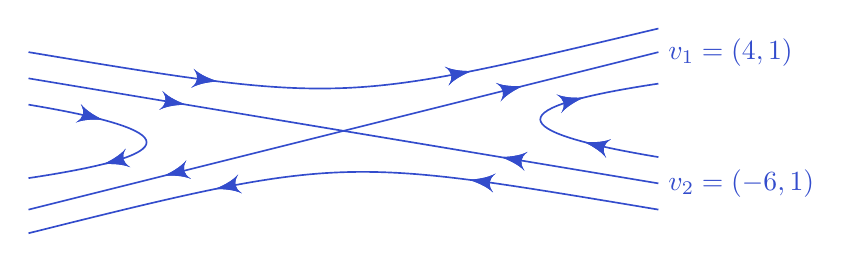
\begin{tikzpicture}
      \draw [->-=0.785, -<-=0.215, mblue, semithick] (-4, -1) -- (4, 1) node [right] {$v_1 = (4, 1)$};
      \draw [->-=0.25, -<-=0.75, mblue, semithick] (-4, 0.667) -- (4, -0.667) node [right] {$v_2 = (-6, 1)$};

      \draw [mblue, semithick, ->- = 0.3, ->- = 0.7] (-4, 1) .. controls (0, 0.333) and (0, 0.35) .. (4, 1.3);
      \draw [mblue, semithick, -<- = 0.3, -<- = 0.7] (-4, -1.3) .. controls (0, -0.3) and (0, -0.333) .. (4, -1);

      \draw [mblue, semithick, ->- = 0.3, ->- = 0.7] (-4, 0.333) .. controls (-2, 0) and (-2, -0.3) .. (-4, -0.6);
      \draw [mblue, semithick, ->- = 0.3, ->- = 0.7] (4, -0.333) .. controls (2, 0) and (2, 0.3) .. (4, 0.6);
    \end{tikzpicture}
  \end{center}

  \item If $\lambda_1, \lambda_2$ are real with $\lambda_1\lambda_2 > 0$. wlog assume $|\lambda_1| \geq |\lambda_2|$. Then the phase portrait is
    \begin{center}
      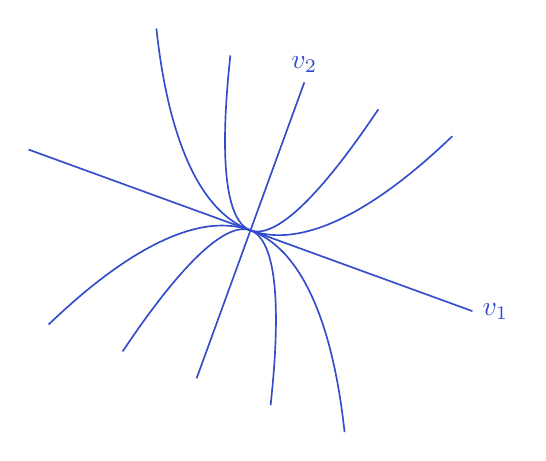
\begin{tikzpicture}[rotate=-20]
        \draw [mblue, semithick] (-3, 0) -- (3, 0) node [right] {$v_1$};
        \draw [mblue, semithick] (0, -2) -- (0, 2) node [above] {$v_2$};

        \draw [mblue, semithick] (-2, 2) parabola bend (0, 0) (2, 2);
        \draw [mblue, semithick] (-1, 2) parabola bend (0, 0) (1, 2);
        \draw [mblue, semithick] (-2, -2) parabola bend (0, 0) (2, -2);
        \draw [mblue, semithick] (-1, -2) parabola bend (0, 0) (1, -2);
      \end{tikzpicture}
    \end{center}
    If both $\lambda_1, \lambda_2 < 0$, then the arrows point towards the intersection and we say there is a stable node. If both are positive, they point outwards and there is an unstable node.

  \item If $\lambda_1, \lambda_2$ are complex conjugates, then we obtain a spiral
    \begin{center}
      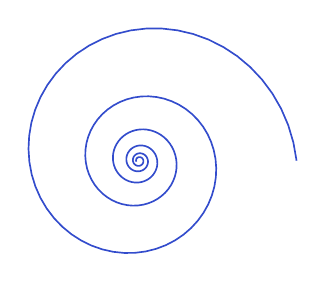
\begin{tikzpicture}
        \draw [mblue, semithick, domain = 0:40,samples=300] plot ({2*exp(-\x/10)*cos(50*\x)}, {2*exp(-\x/10)*sin(50*\x)});
      \end{tikzpicture}
    \end{center}
    If $\re (\lambda_{1, 2}) < 0$, then it spirals inwards. If $\re (\lambda_{1, 2}) > 0$, then it spirals outwards. If $\re (\lambda_{1, 2}) = 0$, then we have ellipses with common centers instead of spirals. We can determine whether the spiral is positive (as shown above), or negative (mirror image of the spiral above) by considering the eigenvectors.
\end{enumerate}

\subsection{Nonlinear dynamical systems}
Consider the second-order autonomous system (ie. $t$ does not explicitly appear in the forcing terms on the right)
\begin{align*}
  \dot x &= f(x, y)\\
  \dot y &= g(x, y)
\end{align*}
It can be difficult to solve the equations, but we can learn a lot about phase-space trajectories of these solutions by studying the equilibria and their stability.

\begin{defi}[Equilibrium point]
  An \emph{equilibrium point} is a point in which $\dot x = \dot y = 0$ at $\mathbf{x}_0 = (x_0, y_0)$.
\end{defi}

Clearly this occurs when $f(x_0, y_0) = g(x_0, y_0) = 0$. We solve these simultaneously for $x_0, y_0$.

To determine the stability, write $x = x_0 + \xi$, $y = y_0 + \eta$. Then
\begin{align*}
  \dot \xi &= f(x_0 + \xi, y_0 + \eta)\\
  &= f(x_0, y_0)+ \xi \frac{\partial f}{\partial x}(\mathbf{x}_0) + \eta \frac{\partial f}{\partial y}(\mathbf{x}_0) + O(\xi^2, \eta^2)
\end{align*}
So if $\xi, \eta \ll 1$,
\[
  \begin{pmatrix}
    \dot \xi\\\dot \eta
  \end{pmatrix} =
  \begin{pmatrix}
    f_x & f_y\\
    g_x & g_y
  \end{pmatrix}
  \begin{pmatrix}
    \xi\\\eta
  \end{pmatrix}
\]
This is a linear system, and we can determine its character from the eigensolutions.

\begin{eg}
  (Population dynamics - predator-prey system) Suppose that there are $x$ prey and $y$ predators. Then we have the following for the prey:
  \[
    \dot x = \underbrace{\alpha x}_{\text{births - deaths}} - \underbrace{\beta x^2}_{\text{natural competition}} - \underbrace{\gamma xy}_{\text{killed by predators}}.
  \]
  and the following for the predators:
  \[
    \dot y = \underbrace{\varepsilon xy}_{\text{birth/survival rate}} - \underbrace{\delta y}_{\text{natural death rate}}
  \]
  For example, let
  \begin{align*}
    \dot x &= 8x - 2x^2 - 2xy\\
    \dot y &= xy - y
  \end{align*}
  We find the fixed points: $x(8 - 2x - 2y) = 0$ gives $x = 0$ or $y = 4 - x$.

  We also want $y(x - 1) = 0$ which gives $y = 0$ or $x = 1$.

  So the fixed points are $(0, 0), (4, 0), (1, 3)$.

  Near $(0, 0)$, we have
  \[
    \begin{pmatrix}
      \dot \xi\\\dot \eta
    \end{pmatrix}=
    \begin{pmatrix}
      8 & 0\\
      0 & -1
    \end{pmatrix}
    \begin{pmatrix}
      \xi\\
      \eta
    \end{pmatrix}
  \]
  We clearly have eigenvalues $8, -1$ with the standard basis as the eigenvectors.
  \begin{center}
    \begin{tikzpicture}[scale = 0.7]
      \draw [<->] (-2, 0) -- (2, 0);
      \draw (2, 0) -- (3, 0);
      \draw (-2, 0) -- (-3, 0);

      \draw [->] (0, 2) -- (0, 1.4);
      \draw (0, 1.4) -- (0, -1.4);
      \draw [->] (0, -2) -- (0, -1.4);
    \end{tikzpicture}
  \end{center}
  Near $(4, 0)$, we have $x = 4 + \xi$, $y = \eta$. Instead of expanding partial derivatives, we can obtain from the equations directly:
  \begin{align*}
    \dot\xi &= (4 + \xi)(8 - 8 - 2\xi - 2\eta)\\
    &= - 8\xi - 8\eta -2\xi^2 - 2\xi\eta\\
    \dot\eta &= \eta(4 + \xi - 1)\\
    &= 3\eta + \xi\eta
  \end{align*}
  Ignoring the second-order terms, we have
  \[
    \begin{pmatrix}
      \dot\xi\\\dot\eta
    \end{pmatrix} =
    \begin{pmatrix}
      -8 & -8 \\
      0 & 3\\
    \end{pmatrix}
    \begin{pmatrix}
      \xi\\\eta
    \end{pmatrix}
  \]
  The eigenvalues are $-8$ and $3$, with associated eigenvectors $(1, 0), (8, -11)$.
  \begin{center}
    \begin{tikzpicture}[scale = 0.7]
      \draw (-2, 0) -- (2, 0);
      \draw [<-] (2, 0) -- (3, 0);
      \draw [<-] (-2, 0) -- (-3, 0);

      \draw (-1, 2) -- (-.7, 1.4);
      \draw [<->](-.7, 1.4) -- (.7, -1.4);
      \draw (1, -2) -- (.7, -1.4);
    \end{tikzpicture}
  \end{center}
  Near $(1, 3)$, we have $x = 1 + \xi, y = 3 + \eta$. So
  \begin{align*}
    \dot \xi &= (1 + \xi)(8 - 2 - 2\xi - 6 - 2\eta)\\
    &\approx -2\xi - 2\eta\\
    \dot\eta &= (3 + \eta)(1 + \xi - 1)\\
    &\approx 3\eta
  \end{align*}
  So
  \[
    \begin{pmatrix}
      \dot\xi\\\dot\eta
    \end{pmatrix} =
    \begin{pmatrix}
      -2 & -2\\
      3 & 0
    \end{pmatrix}
    \begin{pmatrix}
      \xi\\\eta
    \end{pmatrix}
  \]
  The eigenvalues are $- 1\pm i\sqrt{5}$. Since it is complex with a negative real part, it is a stable spiral.

  We can determine the chirality of the spirals by considering what happens to a small perturbation to the right $
  \begin{pmatrix}
    \xi\\0
  \end{pmatrix}$ with $\xi > 0$. We have $
  \begin{pmatrix}
    \dot\xi\\\dot\eta
  \end{pmatrix} =
  \begin{pmatrix}
    -2\xi\\3\xi
  \end{pmatrix}$. So $\mathbf{x}$ will head top-left, and the spiral is counter-clockwise (``positive'').

  We can patch the three equilibrium points together and obtain the following phase portrait:
  \begin{center}
    \includegraphics[width=180pt]{images/de_population_phase.pdf}
  \end{center}
  We see that $(1, 3)$ is a stable solution in which almost all solutions spiral towards.
\end{eg}

\section{Partial differential equations (PDEs)}
\subsection{First-order wave equation}
Consider the equation of the form
\[
  \frac{\partial y}{\partial t} = c\frac{\partial y}{\partial x},
\]
with $c$ a constant and $y$ a function of $x$ and $t$. This is known as the \emph{(first-order) wave equation}. We will later see that solutions correspond to waves travelling in one direction.

We write this as
\[
  \frac{\partial y}{\partial t} - c\frac{\partial y}{\partial x} = 0.
\]
Recall that along a path $x = x(t)$ so that $y = y(x(t), t)$,
\begin{align*}
  \frac{\d y}{\d t} &= \frac{\partial y}{\partial x}\frac{\d x}{\d t} + \frac{\partial y}{\partial t}\\
  &= \frac{\d x}{\d t}\frac{\partial y}{\partial x} + c\frac{\partial y}{\partial x}
\end{align*}
by the chain rule. Now we choose a path along which
\[
  \frac{\d x}{\d t} = -c. \tag{1}
\]
Along such paths,
\[
  \frac{\d y}{\d t} = 0 \tag{2}
\]
So we have replaced the original partial differential equations with a pair of ordinary differential equations.

Each path that satisfies (1) can be described by $x = x_0 - ct$, where $x_0$ is a constant. We can write this as $x_0 = x + ct$.

From (2), along each of these paths, $y$ is constant. So suppose for each $x_0$, the value of $y$ along the path $x_0 = x + ct$ is given by $f(x_0)$, where $f$ is an arbitrary function. Then the solution to the wave equation is
\[
  y = f(x + ct),
\]
By differentiating this directly, we can easily check that every function of this form is a solution to the wave equation.

The contours of $y$ look rather boring.
\begin{center}
  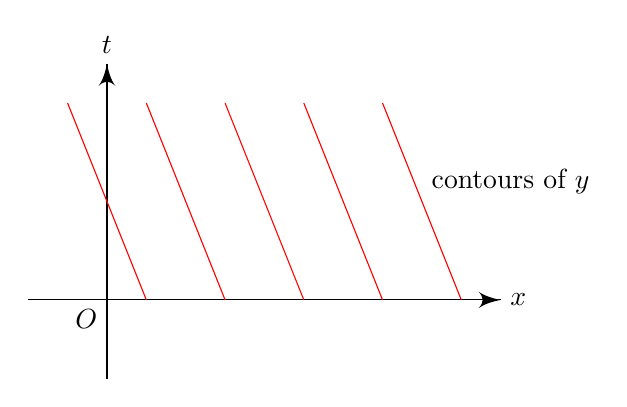
\begin{tikzpicture}
    \draw [->] (-1, 0) -- (5, 0) node [right] {$x$};
    \draw [->] (0, -1) -- (0, 3) node [above] {$t$};
    \node [anchor = north east] at (0, 0) {$O$};

    \foreach \x in {1, 2, 3, 4, 5} {
      \draw [red] (\x- 0.5, 0) -- (\x - 1.5, 2.5);
    }
    \node [right] at (4, 1.5) {contours of $y$};
  \end{tikzpicture}
\end{center}
Note that as we move up the time axis, we are simply taking the $t = 0$ solution and translating it to the left.

The paths we've identified are called the ``characteristics'' of the wave equation. In this particular example, $y$ is constant along the characteristics (because the equation is unforced).

We usually have initial conditions eg.
\[
  y(x, 0) = x^2 - 3
\]
Since we know that $y = f(x + ct)$ and $f(x) = x^2 - 3$, $y$ must be given by
\[
  y = (x + ct)^2 - 3.
\]
We can plot the $xy$ curve for different values of $t$ to obtain this:
\begin{center}
  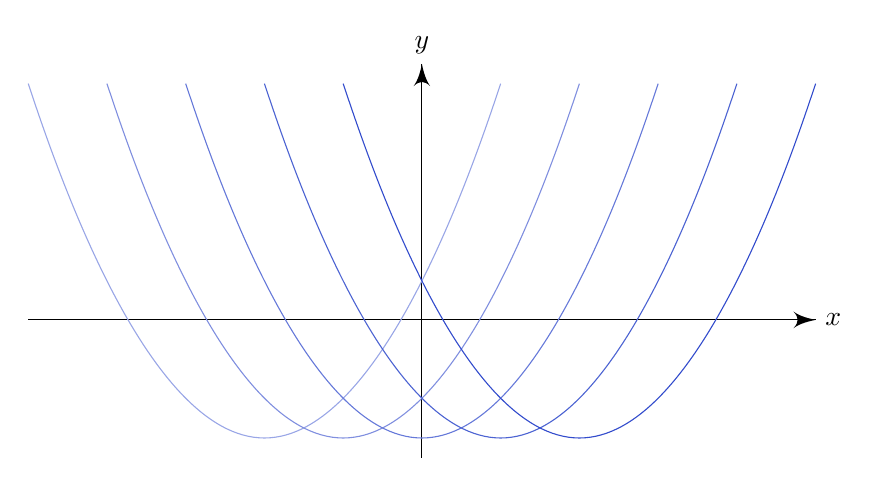
\begin{tikzpicture}[yscale=0.5]
    \draw [->] (-5, 0) -- (5, 0) node [right] {$x$};
    \draw [->] (0, -3.5) -- (0, 6.5) node [above] {$y$};

    \foreach \t in {-2,...,2}{
      \pgfmathsetmacro\k{(\t + 6) * 12.5}
      \draw [mblue!\k] (3 + \t ,6) parabola bend (\t , -3) (- 3 + \t, 6);
    }
  \end{tikzpicture}
\end{center}
We see that each solution is just a translation of the $t = 0$ version.

We can also solve forced equations, such as
\[
  \frac{\partial y}{\partial t} + 5\frac{\partial y}{\partial x} = e^{-t},\quad y(x, 0) = e^{-x^2}.
\]
Along each path $x_0 = x - 5t$, we have $\frac{\d y}{\d t} = e^{-t}$. So $y = f(x_0) - e^{-t}$ for some function $f$.

Using the boundary conditions provided, At $t = 0$, $y = f(x_0) - 1$ and $x = x_0$. So $f(x_0) - 1 = e^{-x_0^2}$, ie. $f(x_0) = 1 + e^{-x_0^2}$. So
\[
  y = 1 + e^{-(x - 5t)^2} - e^{-t}.
\]
\subsection{Second-order wave equation}
We consider equations in the following form:
\[
  \frac{\partial ^2 y}{\partial t^2} = c^2 \frac{\partial^2 y}{\partial x^2}.
\]
This is the \emph{second-order wave equation}, and is often known as the ``hyperbolic equation'' because the form resembles that of a hyperbola (which has the form $x^2 - b^2 y^2 = 0$). However, the differential equation has no connections to hyperbolae whatsoever.

This equation models an actual wave in one dimensions. Consider a horizontal string, along the $x$ axis. We let $y(x, t)$ be the vertical displacement of the string at the point $x$ at time $t$.
\begin{center}
  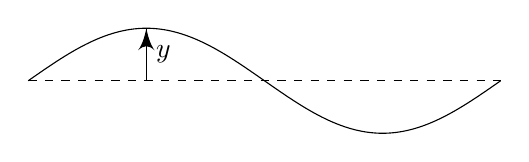
\begin{tikzpicture}
    \draw (0, 0) sin (1.5, 0.667) cos (3, 0) sin (4.5, -0.667) cos (6, 0);
    \draw [dashed] (0, 0) -- (6, 0);
    \draw [->] (1.5, 0) -- (1.5, 0.667) node [pos = 0.5, right] {$y$};
  \end{tikzpicture}
\end{center}
Suppose that $\rho(x)$ is the mass per unit length of a string. Then the restoring force on the string $\displaystyle ma = \rho \frac{\partial ^2 y}{\partial t^2}$ is proportional to the second derivative $\displaystyle\frac{\partial^2 y}{\partial x^2}$. So we obtain this wave equation.

(Why is it proportional to the second derivative? It certainly cannot be proportional to $y$, because we get no force if we just move the whole string upwards. It also cannot be proportional to $\partial y/\partial x$: if we have a straight slope, then the force pulling upwards is the same as the force pulling downwards, and we should have no force. We have a force only if the string is curved, and curvature is measured by the second derivative)

To solve the equation, suppose that $c$ is constant. Then we can write
\begin{align*}
  \frac{\partial ^2 y}{\partial t^2} - c^2 \frac{\partial^2 y}{\partial x^2} &= 0\\
  \left(\frac{\partial}{\partial t} + c\frac{\partial}{\partial x}\right)\left(\frac{\partial}{\partial t} - c\frac{\partial}{\partial x}\right) y &= 0
\end{align*}
If $y = f(x + ct)$, then the first operator differentiates it to give a constant (as in the first-order wave equation). Then applying the second operator differentiates it to $0$. So $y = f(x + ct)$ is a solution.

Since the operators are commutative, $y = f(x - ct)$ is also a solution. Since the equation is linear, the general solution is
\[
  y = f(x + ct) + g(x - ct).
\]
This shows that the solution composes of superpositions of waves travelling to the left and waves travelling to the right.

We can show that this is indeed the most general solution by substituting $\xi = x + ct$ and $\eta = x - ct$. We can show, using the chain rule, that $y_{tt} - c^2 y_{xx} \equiv -4c^2 y_{\eta\xi} = 0$. Integrating twice gives $y = f(\xi) + g(\eta)$.

How many boundary conditions do we need to have a unique solution? In ODEs, we simply count the order of the equation. In PDEs, we have to count over all variables. In this case, we need 2 boundary conditions and 2 initial conditions. For example, we can have:
\begin{itemize}
  \item Initial conditions: at $t = 0$,
    \begin{gather*}
      y = \frac{1}{1 + x^2}\\
      \frac{\partial y}{\partial t} = 0
    \end{gather*}
  \item Boundary conditions: $y \to 0$ as $x \to \pm \infty$.
\end{itemize}
We know that the solution has the form
\[
  y = f(x + ct) + g(x - ct).
\]
The first initial condition give
\[
  f(x) + g(x) = \frac{1}{1 + x^2}\tag{1}
\]
The second initial condition gives
\[
  \frac{\partial y}{\partial t} = cf'(x) - cg'(x)\tag{2} = 0
\]
From (2), we know that $f' = g'$. So $f$ and $g$ differ by a constant. wlog, we can assume that they are indeed equal, since if we had, say, $f = g + 2$, then we can let $y = (f(x + ct) + 1) + (g(x - ct) + 1)$ instead, and the new $f$ and $g$ are equal.

From (1), we must have
\[
  f(x) = g(x) = \frac{1}{2(1 + x^2)}
\]
So, overall,
\[
  y = \frac{1}{2}\left[\frac{1}{1 + (x + ct)^2} + \frac{1}{1 + (x - ct)^2}\right]
\]
Where we substituted $x$ for $x +ct$ and $x - ct$ in $f$ and $g$ respectively.

\subsection{The diffusion equation}
Heat conduction in a solid in one dimension is modelled by the diffusion equation
\[
  \frac{\partial T}{\partial t} = \kappa \frac{\partial^2 T}{\partial x^2}
\]
This is known as a parabolic PDE (parabolic because it resembles $y = ax^2$).

Here $T(x, t)$ is the temperature and the constant $\kappa$ is the \emph{diffusivity}.

\begin{eg}
  Consider an infinitely long bar heated at one end ($x = 0$). Note in general the ``velocity'' $\partial T/\partial t$ is proportional to curvature $\partial^2 T/\partial x^2$, while in the wave equation, it is the ``acceleration'' that is proportional to curvature. In this case, instead of oscillatory, the diffusion equation is dissipative and all unevenness simply decays away.

  Suppose $T(x,0) = 0$, $T(0, t) = H(t) =
  \begin{cases}
    0 & t < 0\\
    1 & t > 0
  \end{cases}$, and $T(x, t)\to 0$ as $x\to \infty$. In words, this says that the rod is initially cool (at temperature $0$), and then the end is heated up on one end after $t = 0$.

  There is a \emph{similarity solution} of the diffusion equation valid on an infinite domain (or our semi-infinite domain) in which $T(x, t) = \theta(\eta)$, where $\displaystyle \eta = \frac{x}{2\sqrt{\kappa t}}$.

  Applying the chain rule, we have
  \begin{align*}
    \frac{\partial T}{\partial x} &= \frac{\d \theta}{\d \eta} \frac{\partial \eta}{\partial x}\\
    &= \frac{1}{2\sqrt{\kappa t}} \theta'(\eta)\\
    \frac{\partial^2 T}{\partial x^2} &= \frac{1}{2\sqrt{\kappa t}} \frac{\d\theta'}{\d\eta}\frac{\partial \eta}{\partial x}\\
    &= \frac{1}{4\kappa t}\theta''(\eta)\\
    \frac{\partial T}{\partial t} &= \frac{\d \theta}{\d \eta}\frac{\partial \eta}{\partial t}\\
    &= -\frac{1}{2}\frac{x}{2\sqrt{\kappa}}\frac{1}{t^{3/2}} \theta'(\eta)\\
    &= -\frac{\eta}{2t}\theta'(\eta)
  \end{align*}
  Putting this into the diffusion equation yields
  \begin{align*}
    -\frac{\eta}{2t}\theta' &= \kappa \frac{1}{4\kappa t}\theta''\\
    \theta'' + 2\eta\theta' &= 0
  \end{align*}
  This is an ordinary differential equation for $\theta(\eta)$. This can be seen as a first-order equation for $\theta'$ with non-constant coefficients. Use the integrating factor $\mu = \exp(\int 2\eta \;\d \eta) = e^{\eta^2}$. So
  \begin{align*}
    (e^{\eta^2}\theta')' &= 0\\
    \theta' &= Ae^{-\eta^2}\\
    \theta &= A\int_0^\eta e^{-u^2}\;\d u + B\\
    &= \alpha\erf(\eta) + B
  \end{align*}
  where $\erf(\eta) = \frac{2}{\sqrt{\pi}} \int_0^\eta e^{-u^2}\;\d u$ from statistics, and $\erf(\eta)\to 1$ as $\eta\to \infty$.

  Now look at the boundary and initial conditions, (recall $\eta = x/(2\sqrt{\kappa t})$) and express them in terms of $\eta$. As $x \to 0$, we have $\eta \to 0$. So $\theta = 1$ at $\eta = 0$.

  Also, if $x\to \infty, t\to 0^+$, then $\eta \to \infty$. So $\theta \to 0$ as $\eta \to \infty$.

  So $\theta(0) = 1 \Rightarrow B = 1$. Colloquially, $\theta(\infty) = 0$ gives $\alpha = -1$. So $\theta = 1 - \erf(\eta)$. This is also sometimes written as $\erfc(\eta)$, the error function complement of $\eta$. So
  \[
    T = \erfc\left(\frac{x}{2\sqrt{\kappa t}}\right)
  \]
  In general, at any particular fixed time $t_0$, $T(x)$ looks like
  \begin{center}
    \begin{tikzpicture}[xscale=3]
      \draw [->] (0, 0) -- (2.1, 0) node [right] {$x$};
      \draw [->] (0, 0) -- (0, 3) node [above] {$T$};

      % approximation of error function
      \draw [mblue, semithick, domain=0:2] plot (\x, {2.5 * (1 + 0.278393 * \x + 0.230389*\x*\x + 0.000972*\x*\x*\x + 0.078108 * \x*\x*\x*\x)^(-4)});
    \end{tikzpicture}
  \end{center}
  with decay length $O(\sqrt{\kappa t})$. So if we actually have a finite bar of length $L$, we can treat it as infinite if $\sqrt{\kappa t} \ll L$, or $t\ll L^2/\kappa$
\end{eg}
\end{document}
